%!TEX root = ../thesis.tex
%*******************************************************************************
%****************************** Third Chapter **********************************
%*******************************************************************************
\chapter{Selection of Heavy Neutral Leptons}
\label{ChapterSelect}

% **************************** Define Graphics Path **************************
\ifpdf
    \graphicspath{{Chapter9/Figs/Raster/}{Chapter9/Figs/PDF/}{Chapter9/Figs/}}
\else
    \graphicspath{{Chapter9/Figs/Vector/}{Chapter9/Figs/}}
\fi

%********************************** %Opening  **************************************

The selection of Heavy Neutral Lepton (HNL) signals from Standard Model (SM) neutrino and cosmic backgrounds using Monte Carlo (MC) is presented.  
MC samples were simulated using the framework detailed in Chapter \ref{ChapterSim} and reconstructed using the framework detailed in Chapter \ref{ChapterReco}.
This is the very first exploration of the Short-Baseline Near Detector (SBND) physics capabilities to search for HNLs, and this selection provides the first benchmark for understanding the current reconstruction performance of HNL signals based on MC.
The selection exploits the boosted topology and late arrival features of HNL signals using the reconstructed charge and light signals from the Time Projection Chamber (TPC) and Photon Detection System (PDS) combined.
%Then, the reconstructed timing resolution is the parameter of interest since the selection relies on the late arrival of HNLs compared to SM neutrinos.
This set up the ground work that can be carried out on data once the detector is operational.

The following chapter covers details on the selection workflow to identify HNL signals from backgrounds.
The foundation of the selection is given in Section \ref{sec:select_intro}, including a description of signals and backgrounds, MC samples and relevant parameters to evaluate to selection.
The first stage of the selection is to reject cosmic backgrounds as discussed in Section \ref{sec:cosmic_rej} and the second stage is to reject SM neutrino backgrounds as discussed in Section \ref{sec:sm_rej}.
Following this, Section \ref{sec:hnl_shower_select} contains details of the last stage of the selection to identify HNL showers from shower-like backgrounds.
The result of the selection procedure is summarised in Section \ref{sec:select_result}.
A discussion of possible improvements in sensitivity with a better timing resolution is given in Section \ref{sec:truth_bucket}.
Finally, some concluding remarks are provided Section \ref{sec:select_conclude}.

%A hypothetical question is proposed in Section \ref{sec:truth_bucket}, driven by the timing resolution observed in reconstruction, concerning whether or not better sensitivity limits can be achieved given an improvement in timing resolution. 
%********************************** %First Section  **************************************

\section{Selection Introduction}
\label{sec:select_intro}

This section provides details of all the ground work before performing the selection. 
Definitions of signals are backgrounds are presented in Section \ref{sec:sig_bkg_def}.
Descriptions of MC samples used in the selection are provided in Section \ref{sec:select_mc}.
Parameters to evaluate the selection, including definitions of efficiency and the arrival time distribution, are detailed in Sections \ref{sec:select_eff} and \ref{sec:key_dist} respectively.

\subsection{Signal and Background Definitions}
\label{sec:sig_bkg_def}

The selection begins with defining the signal topology, namely $\pi^0 \rightarrow \gamma\gamma$ showers resulting from HNLs decaying inside the Fiducial Volume (FV) of the SBND detector.
FV is a smaller volume approximately 70\% of the active volume, to be defined in the forthcoming Section \ref{sec:fv_cut}.
The di-photon showers of HNLs result in one or more showers without any hadronic activities at the vertex.
Fig. \ref{fig:hnl_evd_1shw} shows an event display of two separable photon showers, where each shower can be seen distinctively.
In the case where only a single shower is reconstructed, two scenarios can happen.
The first scenario is that only a single photon deposits energy inside the detector while the other one escapes.
The second scenario is that the di-photon showers are very boosted and forward-going.
Fig. \ref{fig:pi0_distribution} in Section \ref{sec:gen_mevprtl} shows that the angle of $\pi^0$ is very beam-collimated for HNLs in the mass range of 140-260 MeV.
Thus, the resulting di-photon showers can overlap each other, in which case the opening angle between the two showers is too small to be reconstructed as two distinct showers. 
Fig. \ref{fig:hnl_evd_2shw} shows an event display of very boosted di-photons showers, which are likely to be reconstructed as a single energetic shower.

\begin{figure}[ht!]
	\centering
        \begin{subfigure}[b]{0.85\textwidth}  
            \centering 
            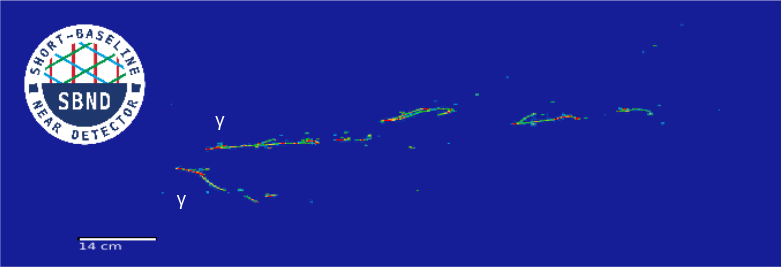
\includegraphics[width=\textwidth]{hnl_2shw}
            \caption{Separable di-photon showers}%
	    \label{fig:hnl_evd_1shw}
        \end{subfigure}
        \centering
        \begin{subfigure}[b]{0.85\textwidth}   
            \centering 
            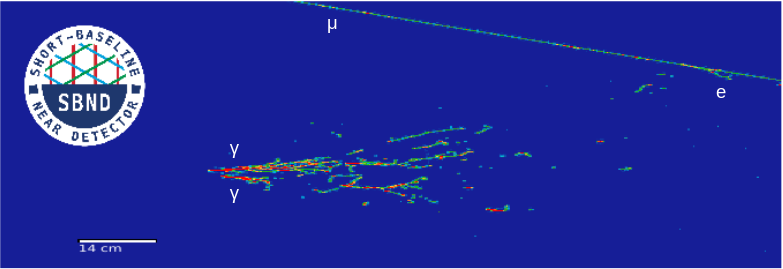
\includegraphics[width=\textwidth]{hnl_1shw}
            \caption{Overlapped di-photon showers}%
	    \label{fig:hnl_evd_2shw}
	\end{subfigure}
	\caption[Event Display of Di-Photon Showers From Heavy Neutral Leptons]{
	Event displays showing two common topologies of simulated di-photon showers from HNLs. 
	}
        \label{fig:hnl_evd_select}
%\end{figure}
%\begin{figure}[hb!]
\vspace{0.5cm}
	\centering
        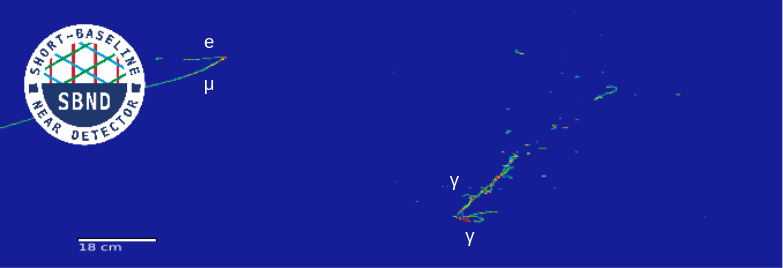
\includegraphics[width=0.85\textwidth]{ncpi0}
        \caption[Event Display of a Neutral Current Interaction Containing a Neutral Pion]{
		Event display showing di-photon showers from a simulated NC $\pi^0$ interaction and a cosmic stopping muon. 
	}
	\label{fig:ncpi0_evd}
\end{figure}

%SM neutrino background
Given this signal topology, the first-order background topology from SM neutrinos is Neutral Current interactions that produce $\pi^0$ (NC $\pi^0$).
This interaction type also produces di-photon showers with little or no hadronic activities at the vertex.
The second-order background topology is from Charged Current electron (anti-)neutrinos (CC $\nu_e$) interactions.
This interaction type typically produces one or multiple hadrons in addition to a single electron shower.
However, in some scenarios, the hadrons are too low in energy to be reconstructed, resulting in a single shower topology after reconstruction.
Fig. \ref{fig:ncpi0_evd} shows an event display of the observable di-photon showers from NC $\pi^0$ interaction, which is indistinguishable from the di-photon showers from HNLs.
The key distinction separating HNL showers from these SM neutrino showers is the boosted topology of HNLs, where HNL di-photon showers have smaller opening angles and tend to travel preferably in the beam direction. 
%and can be exploited for selection to be detailed in Section \ref{sec:hnl_shower_select}.

SM neutrino interactions can occur outside the FV, but their products can have sufficient energy to propagate inside the FV.
Interactions occurring outside the FV but inside the detector volume are referred to as Non-FV interactions.
Interactions occurring completely outside the detector volume are referred to as dirt neutrino interactions.
As previously discussed in Section \ref{sec:gen_genie}, despite interacting outside of the FV, these interactions can introduce non-negligible backgrounds, especially if their products also produce showers in the final states. 

%Cosmic background and CCnumu
%The track signature for protons is short stubs, while the track signature for muons and pions is long tracks.
Finally, any background interactions that produce tracks are considered low-priority backgrounds since a track topology is easily distinguishable from a shower topology.
From SM neutrinos, these interactions are from Charged Current muon (anti-)neutrinos (CC $\nu_\mu$) or any Neutral Current interactions that do not produce a neutral pion (Other NC).
Fig. \ref{fig:numu_cos_evd} shows an event display of a common observable from CC $\nu_\mu$ interactions containing 1 muon and 1 proton in the final state.
Similarly, cosmic muons typically leave very long tracks crossing the entire detector with features of delta rays or Michel electrons (See Sections \ref{sec7:delta} and \ref{sec3:bethebloch}).
Fig. \ref{fig:hnl_evd_2shw} (top right) and Fig. \ref{fig:numu_cos_evd} (bottom left) both show a long cosmic track with some delta rays along the track.
Fig. \ref{fig:ncpi0_evd} (top left) shows a cosmic muon coming to a stop and decaying into a Michel electron.

\begin{figure}[hb!]
	\centering
        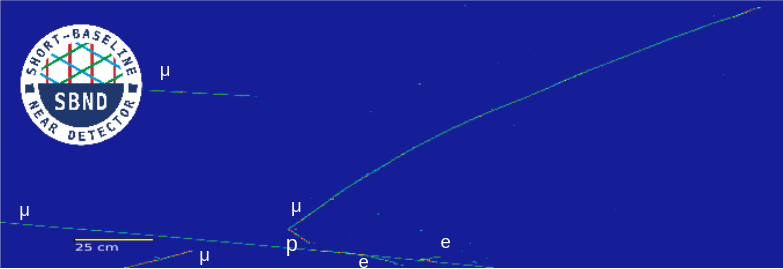
\includegraphics[width=0.85\textwidth]{1m1p_cos}
        \caption[Event Display of a Charged Currect Interaction Containing a Muon and a Proton]{
		Event display showing a muon and a proton track from a simulated CC $\nu_\mu$ interaction together with a few cosmic muons.
	}
	\label{fig:numu_cos_evd}
\end{figure}

%********************************** %First Section  **************************************

\subsection{Description of Monte Carlo Samples}
\label{sec:select_mc}

%The selection presented in this chapter was performed on Monte Carlo (MC) samples, that were generated using the simulation framework described in Chapter \ref{ChapterSim}.
%These samples were then reconstructed using the framework described in Chapter \ref{ChapterReco}.

HNL signals were overlaid with cosmic muons occurring within the TPC readout window.
Samples at the HNL mass of 140, 160, 180, 200, 220, 240 and 260 MeV were generated, totalling 7 samples with 60,000 events per sample.
The number of events per sample can be re-weighted from the simulated coupling $|U_{\mu4}|^{2}$ to another coupling $|U'_{\mu4}|^{2}$ by applying a weight as follows:
\begin{equation}
    w = \left(\frac{|U_{\mu4}|^{2}}{|U'_{\mu4}|^{2}}\right)^{2}.
    \label{eq:reweight_U}
\end{equation}
Eq. \ref{eq:reweight_U} allows for the signal scaling required to perform the limits setting in Chapter \ref{ChapterResult}.   

Three samples of SM neutrinos were also generated.
The first one is a core sample with all SM neutrino interactions occurring inside as well as outside the detector (See Section \ref{sec:gen_genie}).
Two additional dedicated samples of enriched NC $\pi^0$ and CC $\nu_e$ backgrounds were also generated, to improve the limited statistics of these interactions in the core sample.
The three samples were normalised to an exposure of $1 \times 10^{21}$ Protons On Target (POT) to account for 3 years of data taking.
This yields $\sim331,000$ NC $\pi^0$ interactions and $\sim33,000$ CC $\nu_e$ interactions which are the primary background.
Other background from CC $\nu_\mu$ and Other NC interactions make a total of $\sim5$ million interactions.
An additional $\sim2$ million and $\sim3$ million interactions from Non-FV and dirt interactions are also considered as backgrounds, although only a fraction of them deposits energy in the detector.

Finally, a cosmic-only sample was generated to account for in-time cosmics (See Section \ref{sec:gen_corsika}).
This sample consists of events triggered by cosmic-only interactions.
However, it is important to note that a dedicated trigger efficiency study will be carried out to better understand the rate of in-time cosmic events once SBND is operational.
The cosmic-only sample was also normalised to the same POT exposure, and combined with SM neutrino samples to form a single background sample.  

The unit of the selection relies on \textit{events}, where a single event corresponds to a single trigger (See Fig. \ref{fig:SBNDEventStructure} Section \ref{sec:evb}).
After reconstruction, each event contains multiple \textit{slices}, which are interactions reconstructed by Pandora (See Section \ref{sec:pandora}).
A slice consists of a hierarchy of particles starting from the interaction vertex, where each particle can resemble a track or a shower.
The equivalent unit to a slice from the PDS reconstruction is a \textit{flash}, where a flash contains all the light produced from an interaction (See Section \ref{sec:reco_pds}).
The selection is performed on slices, where slices are accepted or rejected based on cuts using the reconstructed information of the slice or by matching a slice to a flash.

%********************************** %First Section  **************************************

\subsection{Selection Efficiency Definition}
\label{sec:select_eff}

For monitoring and quantifying the impacts of selection cuts, selection efficiencies are defined for signals and backgrounds respectively.
The selection efficiency is defined as:
\begin{equation}
	\label{eq:sig_eff}
	\mathrm{Signal\ Efficiency = \frac{Number\ of\ selected\ signal\ slices\ with\ completeness\ >\ 50\ \%}{Number\ of\ signal\ slices\ reconstructed\ as\ neutrinos}}. \\
\end{equation}
In the numerator, the requirement of $> 50\%$ completeness implies that at least 50\% of the slice energy must be deposited by a HNL.
This prevents double counting so that only well-reconstructed signal slices are considered.
In the denominator, the requirement for slices to be reconstructed as neutrinos is embedded by the Pandora workflow.
As stated in Section \ref{sec:pandora}, Pandora performs a cosmic rejection to identify cosmic-like and neutrino-like slices, and only neutrino-like slices are fully reconstructed.
The Pandora cosmic rejection is also employed as the first cosmic cut detailed in Section \ref{sec:cosmic_pandora}.
The denominator describes the starting number of signal slides and the numerator describes the number of selected signal slices.
Thus, Eq. \ref{eq:sig_eff} describes the efficiency of signals remained after selection. 

On the other hand, the background efficiency is defined as:
\begin{equation}
	\label{eq:bkg_eff}
	\mathrm{Background\ Efficiency = \frac{Number\ of\ selected\ background\ slices}{Number\ of\ background\ slices\ reconstructed\ as\ neutrinos}}.
\end{equation}
Here, the background slides comprise both SM neutrino and cosmic slices, that are reconstructed by Pandora as neutrino-like slices.
The denominator describes the starting number of background slides and the numerator describes number of selected background slices. 
Eq. \ref{eq:bkg_eff} therefore describe the efficiency of background slices being selected as signals.

The selection aims for a high background \textit{rejection} without compromising the signal \textit{efficiency}.        
This is equivalent to achieving a low background efficiency defined in Eq. \ref{eq:bkg_eff} and a high signal efficiency defined in Eq. \ref{eq:sig_eff}.
Both efficiencies are discussed for each cut and included in the legends of the upcoming plots.                                                                                             

\subsection{The Arrival Time Distribution}
\label{sec:key_dist}

%The selection workflow was developed by exploiting distinct features of HNLs.
%One previously stated feature is the boosted topology of HNL showers as discussed in Section \ref{sec:sig_bkg_def}.
%It is referred to as the \textit{arrival time distribution} in this work.

The late arrival of HNLs relative to SM neutrinos is previously depicted in Fig. \ref{fig:beam_modulus} in Section \ref{sec:gen_mevprtl}, showing the arrival time distribution of HNLs and SM neutrinos.
The distribution of SM neutrinos resembles a Gaussian-shaped bucket as they travel nearly at the speed of light.
HNLs travel at a slower velocity and smear the Gaussian, resulting in excesses on either sides of the bucket.
This is the key distribution for estimating the sensitivity to HNLs since it demonstrates the distinct shape difference between the signal and the background, to be further discussed in Chapter \ref{ChapterResult}.

To reconstruct the arrival time distribution, the required information is the flash time matched to a slice that corresponds to the start time $t_0$ of the interaction.
The flash time reconstruction using PMT signals is detailed in Sections \ref{sec:reco_pds} with a resolution $\mathcal{O}$(2 ns).
The slice-to-flash matching relies on the level of agreement between reconstructed energy from measured charge and light as summarised in Section \ref{sec:subsystem_match}.

From the interaction time $t_0$, the arrival time at the upstream wall of the detector was computed by shifting from the interaction vertex $z$-position to $z = 0$.
The arrival time corresponds to 81 buckets in a single beam spill.
To overlay 81 buckets as a single one, a modulus equal to the spacing between buckets is applied.
The spacing was measured to be 18.936 by the MicroBooNE experiment \cite{uboone_ns}.
Discussion on different smearing contributors to the arrival time reconstruction is given in Section \ref{sec:truth_bucket}.

The arrival time distributions are shown throughout this chapter to demonstrate the impacts of the selection.
In the following plots, both signals and backgrounds are normalised to the same exposure of $1 \times 10^{21}$ POT.
HNL signals are plotted as a solid red line, with the mass value of 200 MeV and normalised to the coupling $|U_{\mu4}|^2 = 3.16 \times 10^{-7}$.
Components of backgrounds are plotted as a stacked histogram, including NC $\pi^0$ shown in dark blue, Other NC shown in light blue, CC $\nu_{\mu}$ shown in green, CC $\nu_e$ shown in light purple, dirt neutrinos shown in brown and cosmic muons shown in light grey.
The number of slices for each component is also shown in the legend.
The signal and background efficiencies detailed in Section \ref{sec:select_eff} are added at the bottom of the legend.
%The reconstructed arrival time for SM neutrinos resembles a Gaussian with a width of $2.26$ ns as compared to the proton bucket from the Booster synchrotron with an intrinsic width of $1.308$ ns.

%********************************** %First Section  **************************************

\section{Cosmic Background Removal}
\label{sec:cosmic_rej}

Cosmic rejection is the first step of selection, targeting two cosmic components: (1) in-time cosmics occurring inside the beam spill and (2) out-of-time cosmics occurring outside the beam spill but inside the readout window (See Section \ref{sec:gen_corsika}).  
The cosmic removal by Pandora is the first cut, presented in Section \ref{sec:cosmic_pandora}.
The beam spill cut is given in Section \ref{sec:cosmic_spill} and the last cut employing a Boosted Decision Tree (BDT) is provided in Section \ref{sec:cosmic_crumbs}.

\subsection{Pandora Cosmic Removal}
\label{sec:cosmic_pandora}

Being a surface detector, SBND is exposed to a high rate of cosmic rays, expecting $\sim 185$ million reconstructed slices from cosmics for the POT exposure of $1 \times 10^{21}$.
As a comparison, the expected rate of reconstructed slices from SM neutrino interactions is $\sim 11$ million slices.
The first cosmic rejection step targets primarily at removing out-of-time cosmic muons.
As described in Sections \ref{sec:pandora} and \ref{sec:select_eff}, Pandora performs a cosmic removal early in the reconstruction and only neutrino-like slices are fully reconstructed. 
The selection thus begins with selecting only slices reconstructed as a neutrino.
This rejects $90 \%$ of the $\sim 185$ million slices from cosmic, leaving behind only $19.5$ million slices.
Meanwhile, only $0.6 \%$ of the reconstructed slices from HNL signals are removed, with similar reductions across different SM neutrino interactions.  
%The remaining slices after the cut are reconstructed as neutrinos and thus, consist of a reconstructed vertex and dedicated reconstruction algorithms required by the upcoming cuts.

\subsection{Beam Spill Cut}
\label{sec:cosmic_spill}

%implying that each selected slice has a reconstructed flash time .
The second cut to remove cosmics is to consider the flash time of a slice, corresponding to the start time $t_0$ of an interaction. 
Only slices matched to a valid flash are selected and the matched flash time is required to be within the beam spill window.
In the simulation of MC samples, the beam spill window is configured to be between [0.367, 1.967] $\mu$s, with $t = 0\ \mu$s corresponding to the first POT of a beam spill.
Moreover, an interaction can occur anywhere along the 500 cm $z$-length of the detector, equivalent to a smearing of 17 ns in timing.
Thus, the beam spill acceptance window is widened to [0.350, 1.984] $\mu$s.
The beam spill cut is illustrated in Fig. \ref{fig:beamspill_cut}, with the acceptance window shown as dashed red lines.

The cut rejects $4$ million cosmic slices while minimally reducing signal efficiency by $3\%$.
Fig. \ref{fig:bb_beamspill} shows the arrival time distribution after applying the cut, where two components of cosmic rays can be observed.
There is a flat distribution coming from out-of-time cosmics and a very small Gaussian-shaped distribution coming from in-time cosmics.

\begin{figure}[ht!]
        \centering
        \begin{subfigure}[b]{0.495\textwidth}
            \centering
            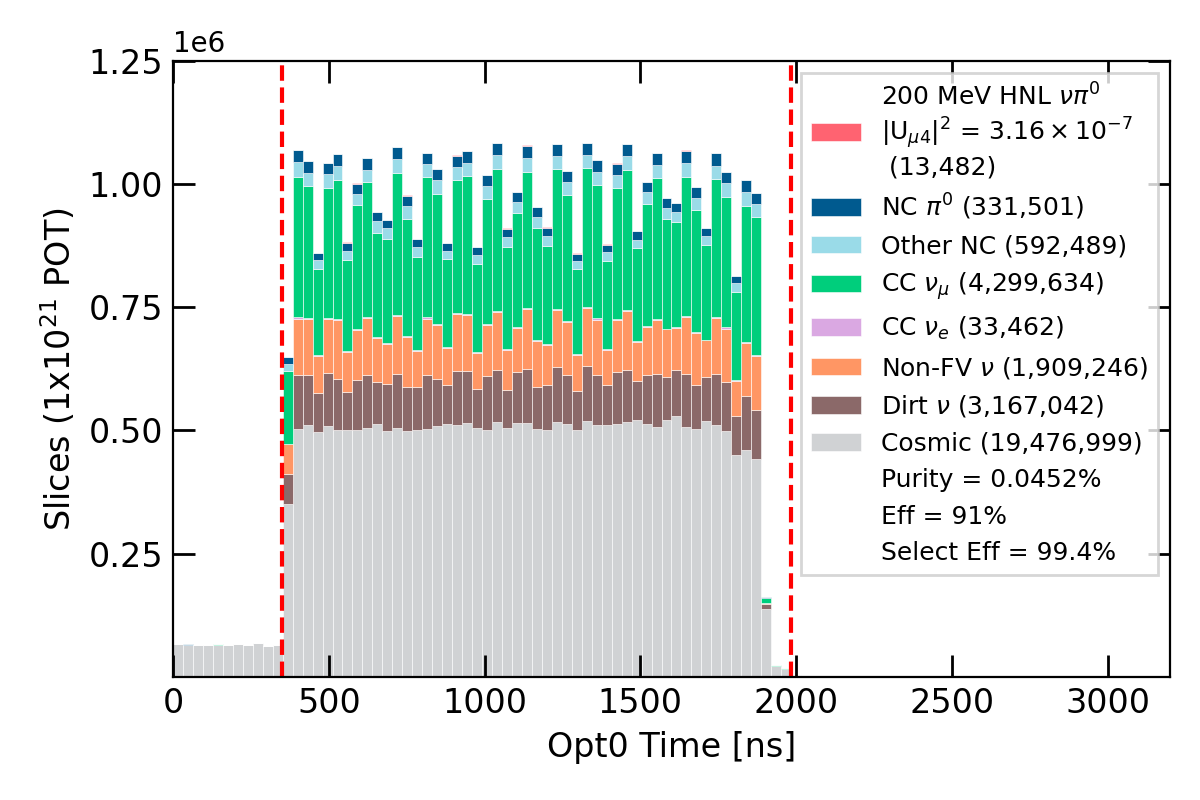
\includegraphics[width=\textwidth]{beamspill}
            \caption{Beam spill cut}%
            \label{fig:beamspill_cut}
        \end{subfigure}
        \hfill
        \begin{subfigure}[b]{0.495\textwidth}  
            \centering 
            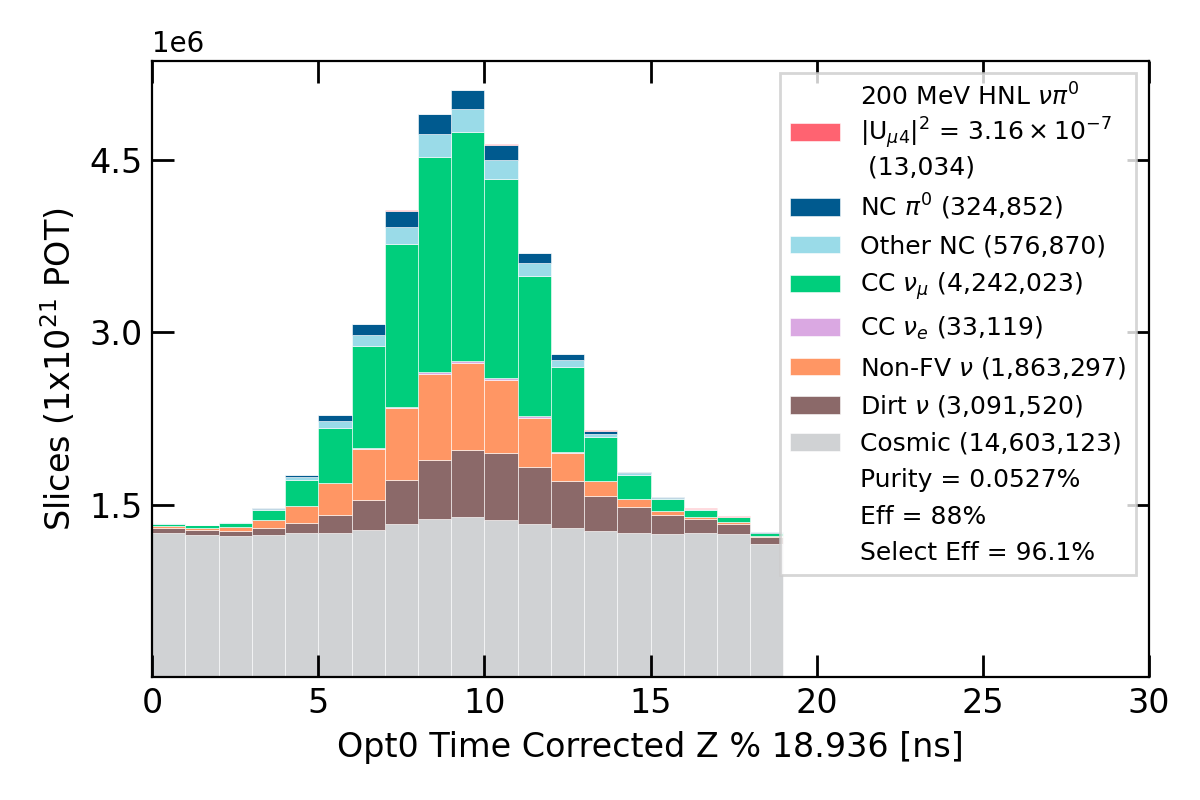
\includegraphics[width=\textwidth]{beam_bucket_post_beamspill}
            \caption{After beam spill cut}%
            \label{fig:bb_beamspill}
        \end{subfigure}
	\caption[Beam Spill Cut]{
		Flash time distribution with the cut (left) and the arrival time distribution after the cut (right). 
	}
        \label{fig:cosmic_bb_cut}
\end{figure}

\subsection{CRUMBS Cut}
\label{sec:cosmic_crumbs}

%given the shower topology is very distinguishable from cosmic tracks.
The third cut targets the out-of-time cosmic components by employing the CRUMBS score of a slice, which is scored by a BDT to distinguish between a neutrino-like slice and a cosmic-like slice (See Section \ref{sec:crumbs}). 
The score distribution of CRUMBS is plotted in Fig. \ref{fig:crumbs_cut}, showing a good separation between neutrino-like and cosmic-like.
A cut is placed to reject any slices with CRUMBS scores less than 0, effectively removing $14$ million of the remaining cosmic slices.

Comparison the arrival time distribution before and after the CRUMBS cut, Fig. \ref{fig:bb_beamspill} and \ref{fig:bb_crumbs}, demonstrates that the majority of the removed cosmics are the out-of-time component. 
The remaining cosmic slices are the in-time component, concentrating at the centre of the arrival time distribution.  
This cut results in an effective background rejection as the background efficiency reduces more than half from $8.3 \times 10^{-1}$ to $3.0 \times 10^{-1}$, whilst the signal efficiency only drops by $5 \%$.
By the end of the cosmic rejection, only $\sim432,000$ of the starting $185$ million cosmic slices remain, equivalent to a $99.9\%$ removal of the cosmic background alone.

\begin{figure}[ht!]
        \begin{subfigure}[b]{0.495\textwidth}   
            \centering 
            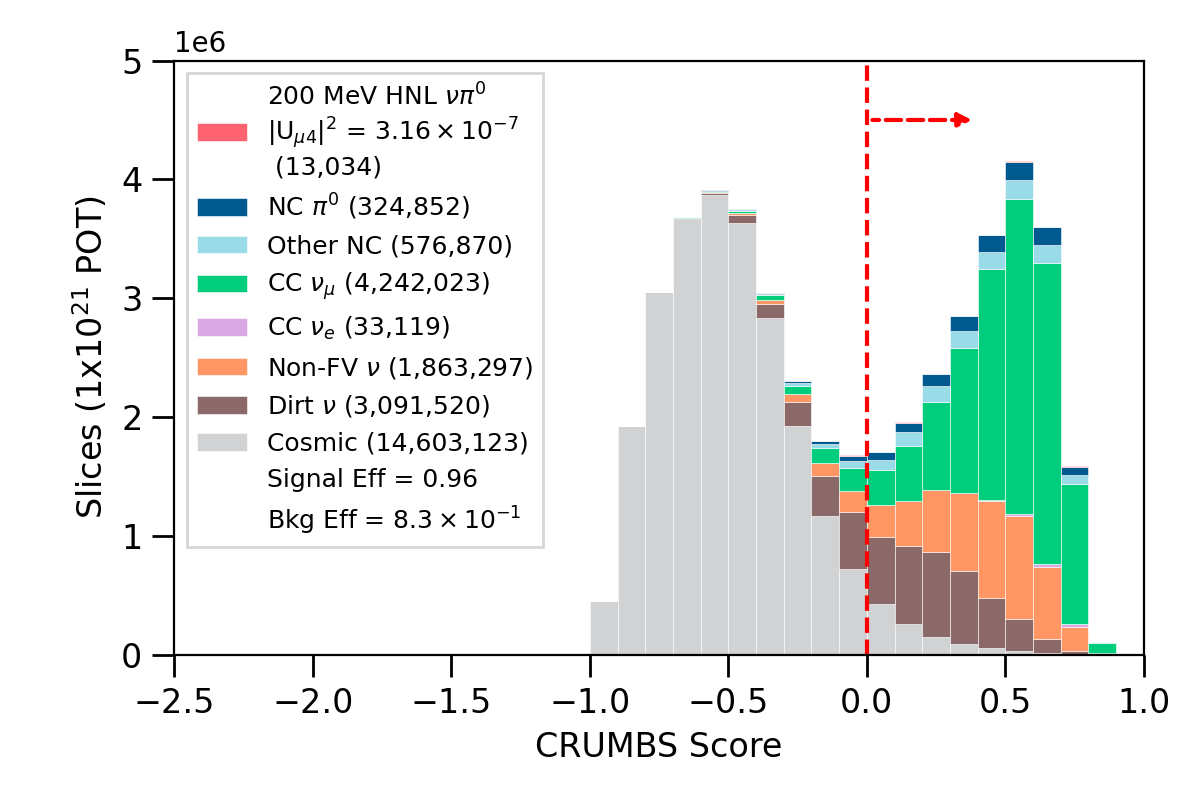
\includegraphics[width=\textwidth]{crumbs_precut}
            \caption{CRUMBS cut}%
            \label{fig:crumbs_cut}
        \end{subfigure}
        \hfill
        \begin{subfigure}[b]{0.495\textwidth}   
            \centering 
            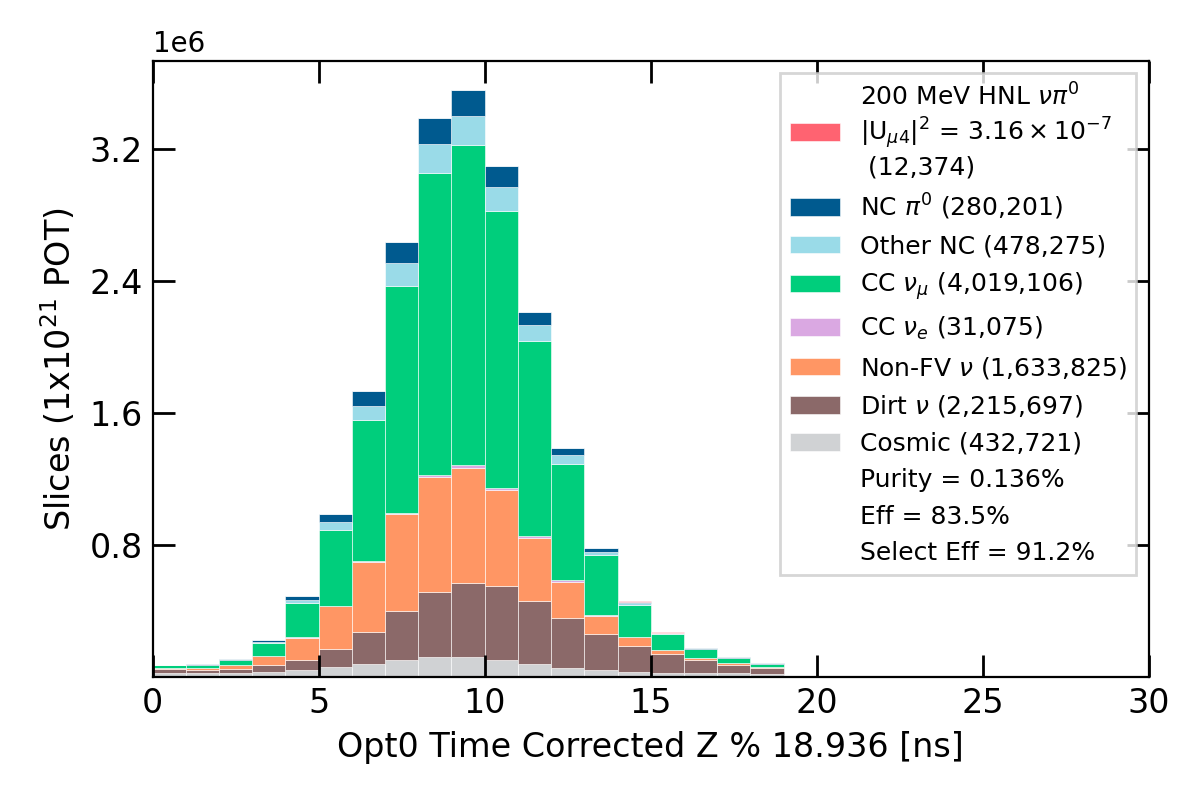
\includegraphics[width=\textwidth]{beam_bucket_post_crumbs}
            \caption{After CRUMBS cut}%
            \label{fig:bb_crumbs}
        \end{subfigure}
	\caption[CRUMBS Cut]{
		CRUMBS score distribution with the cut (left) and the arrival time distribution after the cut (right). 
	}
        \label{fig:cosmic_crumbs_cut}
\end{figure}


\section{Neutrino Background Removal}
\label{sec:sm_rej}

The next set made up of three cuts focusing on rejecting backgrounds of SM neutrinos.
The cut on detector volume is presented Section \ref{sec:fv_cut}.
The cut on the reconstruction quality is detailed in Section \ref{sec:hit_cut}.
Finally, the cut targeting at removing track-like particles from SM neutrino interactions is provided in Section \ref{sec:trk_cut}.

\subsection{Fiducial Volume Cut}
\label{sec:fv_cut}

The cut on detector volume aims to remove backgrounds from Non-FV neutrinos and dirt neutrinos that interact outside of the FV but their products can deposit energy inside the FV. 
The cut requires the reconstructed vertex of a slice to be inside the FV, which is approximately 70\% of the entire active volume of the detector. 
The FV is defined as follows:
\begin{itemize}
        \item $x$-position: $- 180 < x < -5 , 5 < x < 180$ cm,
        \item $y$-position: $-180 < y < 180$ cm,
        \item $z$-position: $10 < z < 450$ cm.
\end{itemize}
The boundary is set on the $x$-axis to reject vertices reconstructed close to the anode and cathode.
Vertices close to the cathode means the charge clusters must traverse the full drift distance before reaching the anode for detection, therefore, are more susceptible to detector effects (See Section \ref{sec:edrift}).
Meanwhile, vertices close to the anode might also indicate particles entering from the side of the detector which are likely to be cosmic muons and Non-FV/dirt neutrino backgrounds. 
The boundary on the $y$-axis rejects interactions that might enter the detector from the top like cosmic muons, or bottom like Non-FV/dirt neutrinos.
Finally, the boundary on the $z$-axis for $z > 10$ cm rejects entering particles and $z < 450$ cm requires enough downstream volume for a shower to grow.
Overall, these cuts ensure the quality of reconstruction.

The distribution of vertices reconstructed inside and outside of the FV is shown in Fig. \ref{fig:fv_cut} and the result of the cut is demonstrated in Fig. \ref{fig:bb_post_fv}.
Dirt neutrino slices reduce from $\sim2$ million slices to only $\sim$306,000 slices while Non-FV neutrino slices drop from $\sim$1.6 million slices to only $\sim99,000$ slices.
The cut reduces both the background efficiency and signal efficiency by a third as it is consistent with rejecting $30\%$ of the detector volume.

\begin{figure}[htb]
        \begin{subfigure}[b]{0.495\textwidth}   
            \centering 
            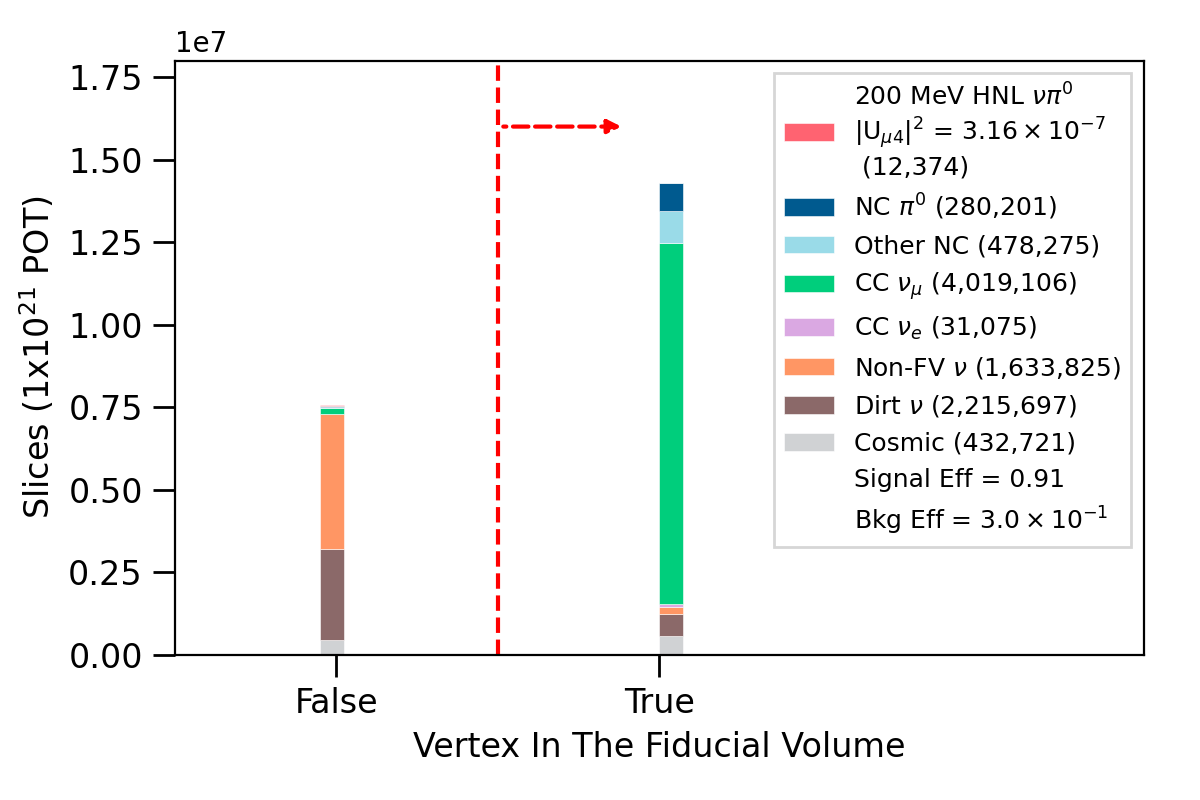
\includegraphics[width=\textwidth]{fv_precut}
            \caption{Fiducial volume cut}%
            \label{fig:fv_cut}
        \end{subfigure}
        \hfill
        \begin{subfigure}[b]{0.495\textwidth}   
            \centering 
            \includegraphics[width=\textwidth]{beam_bucket_post_fv}
            \caption{After fiducial volume cut}%
            \label{fig:bb_post_fv}
        \end{subfigure}
	\caption[Fiducial Volume Cut]{
		Distribution of vertices reconstructed inside and outside of the FV with the cut (left) and the arrival time distribution after the cut (right). 
	}
        \label{fig:quality_fv_cut}
\end{figure}

\subsection{Number of Hits Cut}
\label{sec:hit_cut}

This cut aims to select well-reconstructed slices by examining the number of hits of the primary particle in a slice that deposits the most energy.
The number of hits is particularly important given that Pandora relies on hit information to reconstruct 3D information of particles in a slice (See Sections \ref{sec:signal_process} and \ref{sec:pandora}).
The more hits associated with a particle, the more information is available for Pandora to reconstruct its topology and calorimetry.
The number of hits requirement for the primary particle is $\geq 50$ hits to provide sufficient information for a reliable Pandora reconstruction.
Fig. \ref{fig:Nhits_cut} demonstrates the distribution of the number of hits of the primary particle in a slice. 
Only the first bin is rejected by this cut, demonstrating that only a small amount of slices containing primary particles with $< 50$ hits, which are likely to be poorly reconstructed.
The arrival time distribution after the cut is shown in Fig. \ref{fig:bb_postNhits}, where it can be seen that the cut reduces the signal and background efficiency by < 1\%.

%the cut applied to the full arrival time (left) and only to the first and last 4 bins of the bucket (right).
%Two different distributions of the arrival time were plotted to demonstrate the impact of cut on the full arrival time as well as the edge of the bucket which is the region of interest for HNL search.
%The cut minimally reduces background and signal slices, as can be seen in the plot that the number of rejected slice is small.

\begin{figure}[ht!]
        \begin{subfigure}[b]{0.495\textwidth}   
            \centering 
            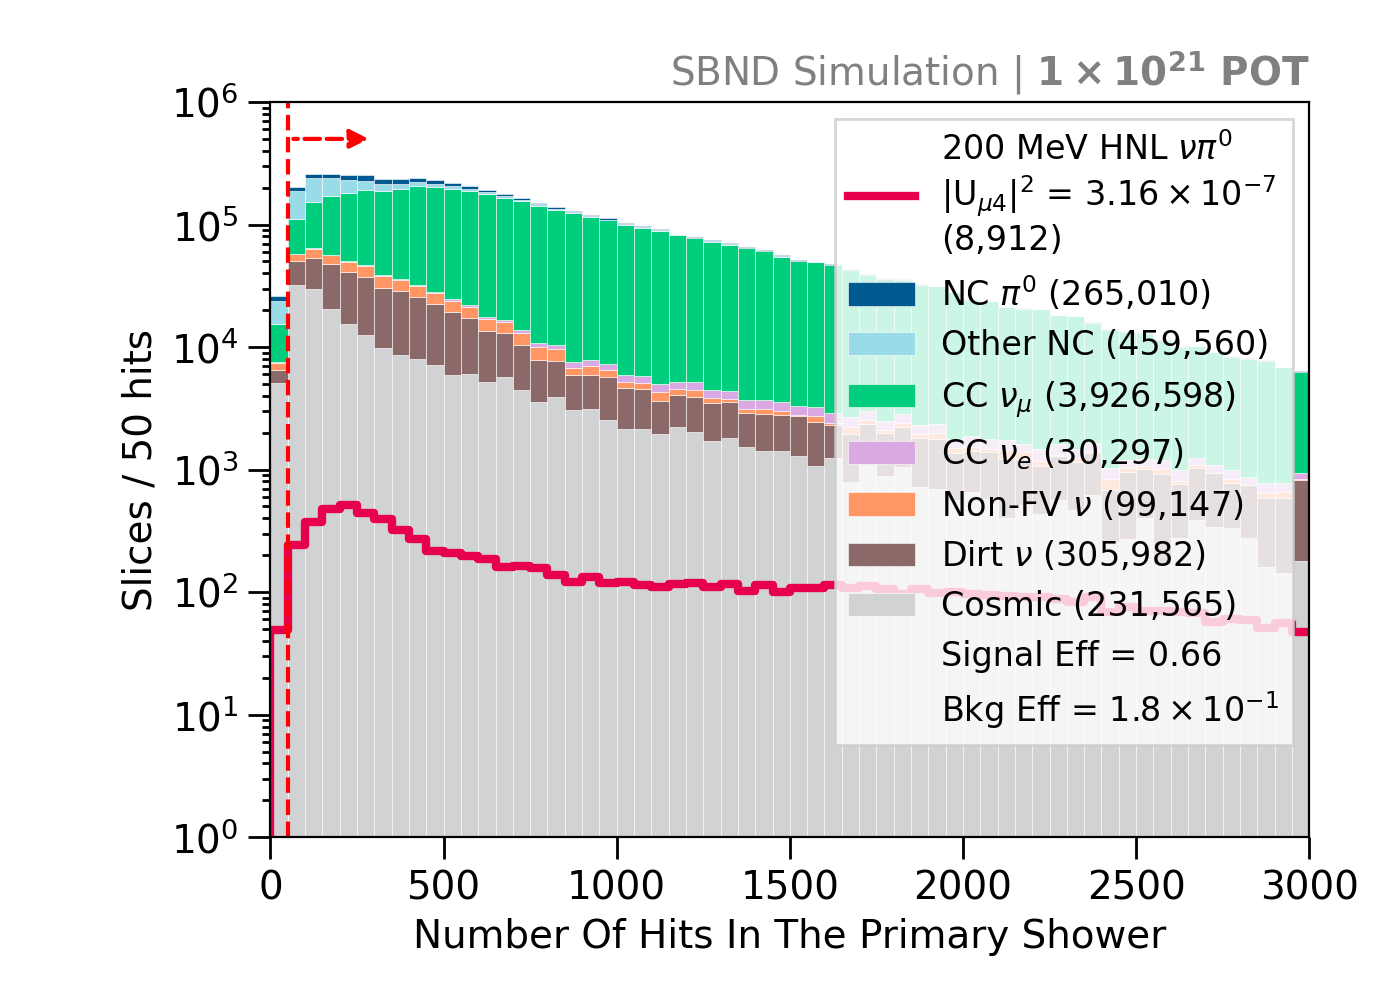
\includegraphics[width=\textwidth]{nHits}
            \caption{Number of hits cut}%
            \label{fig:Nhits_cut}
        \end{subfigure}
        \hfill
        \begin{subfigure}[b]{0.495\textwidth}   
            \centering 
            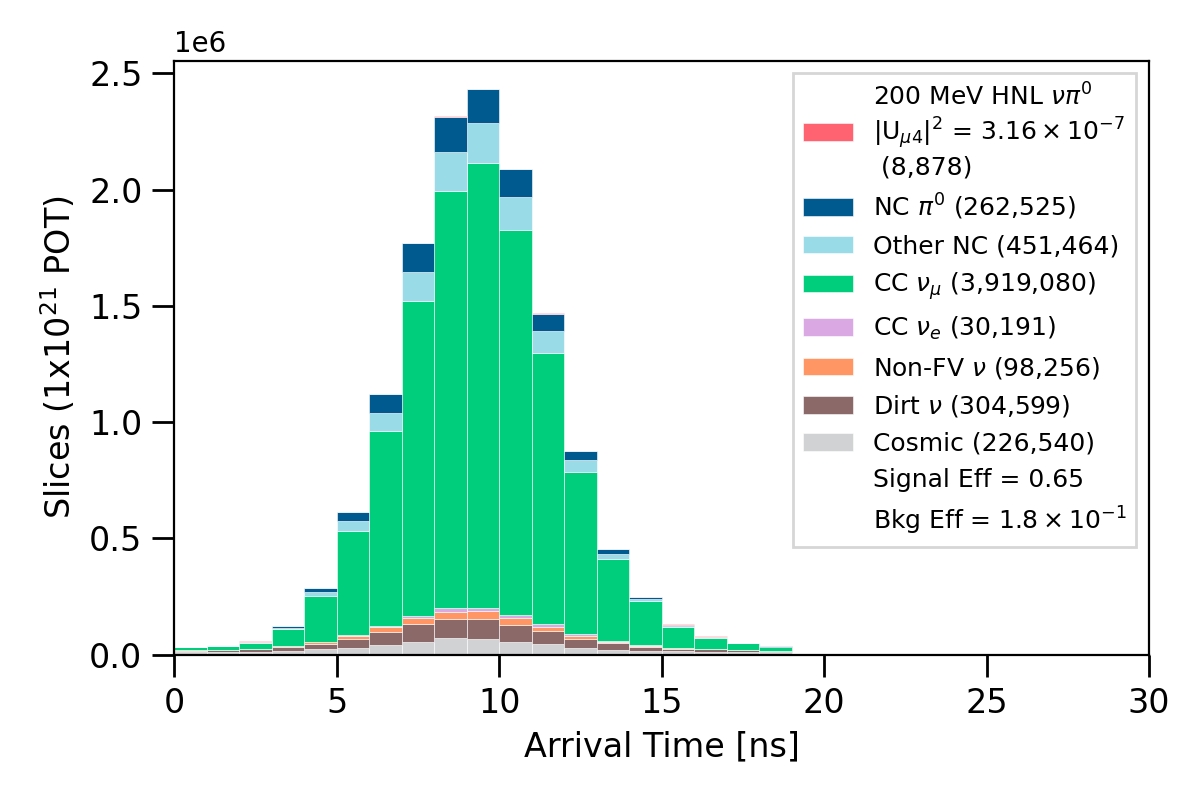
\includegraphics[width=\textwidth]{beam_bucket_postNhits}
            \caption{After number of hits cut}%
            \label{fig:bb_postNhits}
        \end{subfigure}
	\caption[Number of Hits Cut]{
		Number of hits in the primary particle distribution with the cut (left) and the arrival time distribution after the cut (right). 
	}
        \label{fig:quality_hits_cut}
\end{figure}

\subsection{Neutrino Track Removal}
\label{sec:trk_cut}

The next sets of cuts focus on rejecting SM neutrino backgrounds that produce tracks originating from muons, protons and charged pions.
The cut uses the score distribution from the Razzled BDT (See Section \ref{sec:razzled}).
There are two types of Razzled variables examined for this cut: (1) the number of $p, \ \mu, \ \pi$ in a slice as identified by Razzled and (2) the Razzled $p, \ \mu, \ \pi$ scores of all particles in a slice.
The former cut relies on Razzled assigning a type to a particle based on its highest particle type score from the BDT.
The latter cut is to further reject slices if they contain particles with a Razzled score higher than a chosen threshold.

Fig. \ref{fig:nrazzled_muon_full} and \ref{fig:razzled_muon_score_full} demonstrate the two cuts respectively for rejecting muons.
Fig. \ref{fig:nrazzled_muon_full} shows the requirement on the number of Razzled-identified muons is 0 while Fig. \ref{fig:razzled_muon_score_full} shows that only slices containing particles with Razzled muon score $< 0.04$ are selected.
The cuts are very aggressive without compromising signal efficiency due to the distinction between HNL signals and muon tracks.  
Comparison between the arrival time distribution before and after the muon cut, Fig. \ref{fig:bb_postNhits} and Fig. \ref{fig:bb_post_muon}, the muon cut effectively rejects $96\%$ of the $4$ million CC $\nu_\mu$ slices, leaving only $\sim161,000$ slices remaining.
HNL slices are also affected by the cut such that the signal efficiency reduces from 65\% to 51\%.

\begin{figure}[hb!]
        \begin{subfigure}[b]{0.495\textwidth}   
            \centering 
            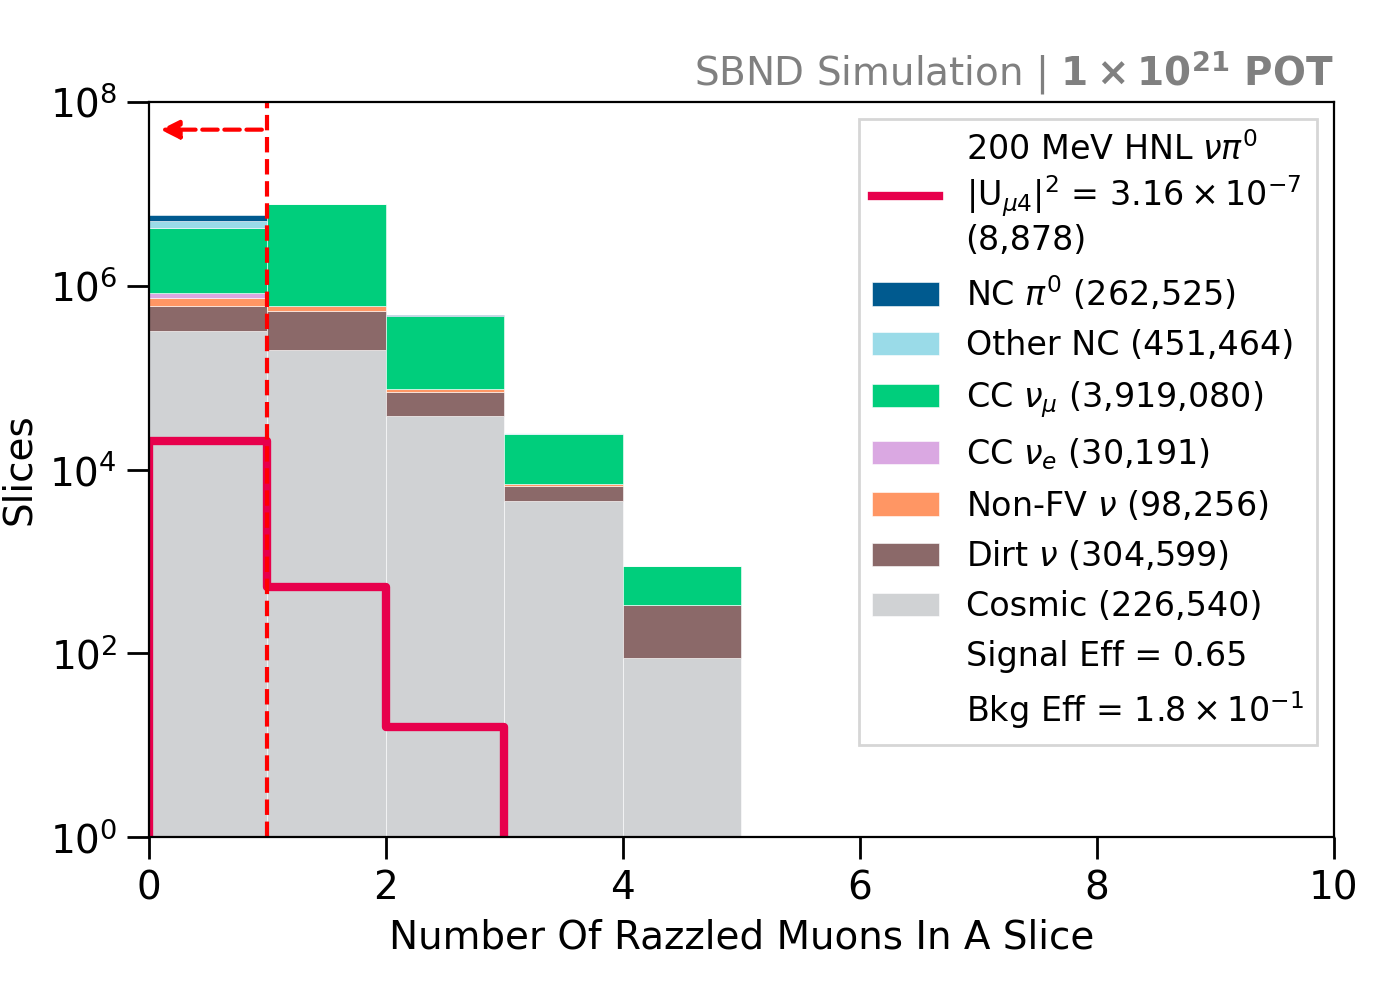
\includegraphics[width=\textwidth]{nrazzled_muon_precut}
            \caption{Number of Razzled-identified muons cut}%
            \label{fig:nrazzled_muon_full}
        \end{subfigure}
        \hfill
        \begin{subfigure}[b]{0.495\textwidth}   
            \centering 
            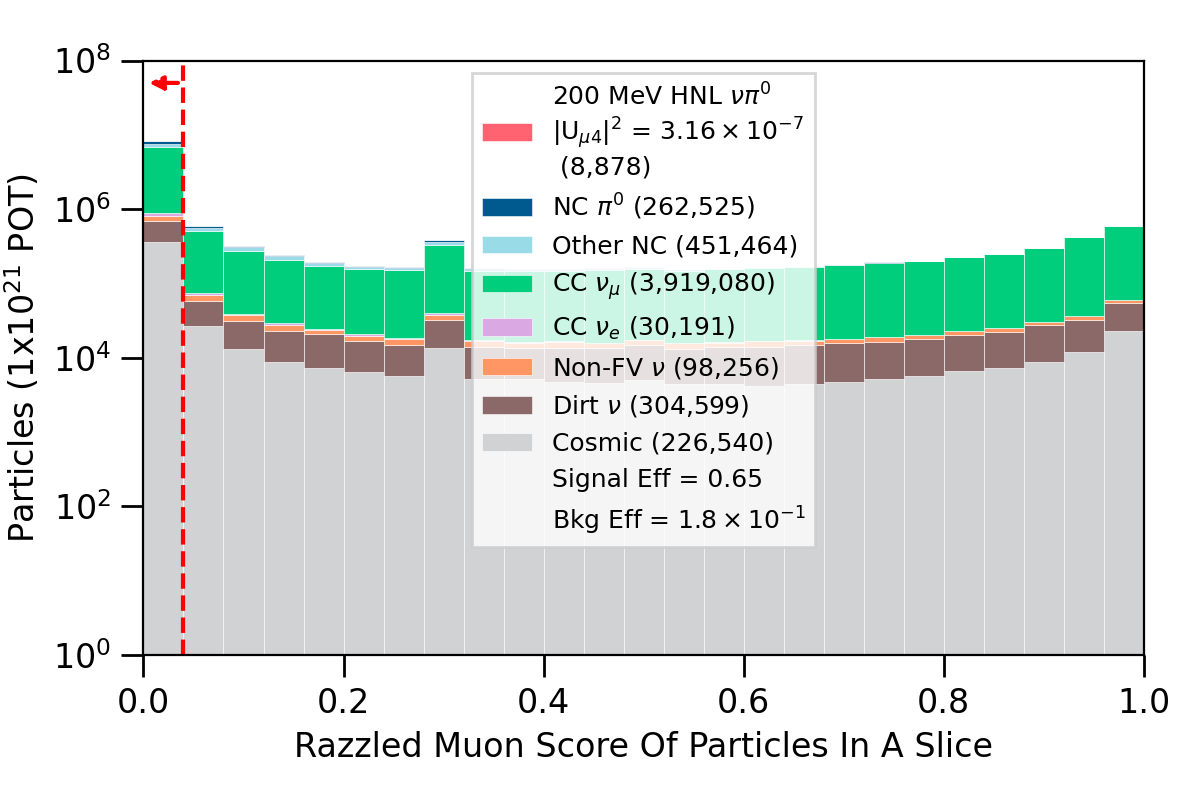
\includegraphics[width=\textwidth]{razzled_muon_score_precut}
            \caption{Particles with Razzled muon score cut}%
            \label{fig:razzled_muon_score_full}
        \end{subfigure}
        \hfill
	\centering
        \begin{subfigure}[b]{0.495\textwidth}   
            \centering 
            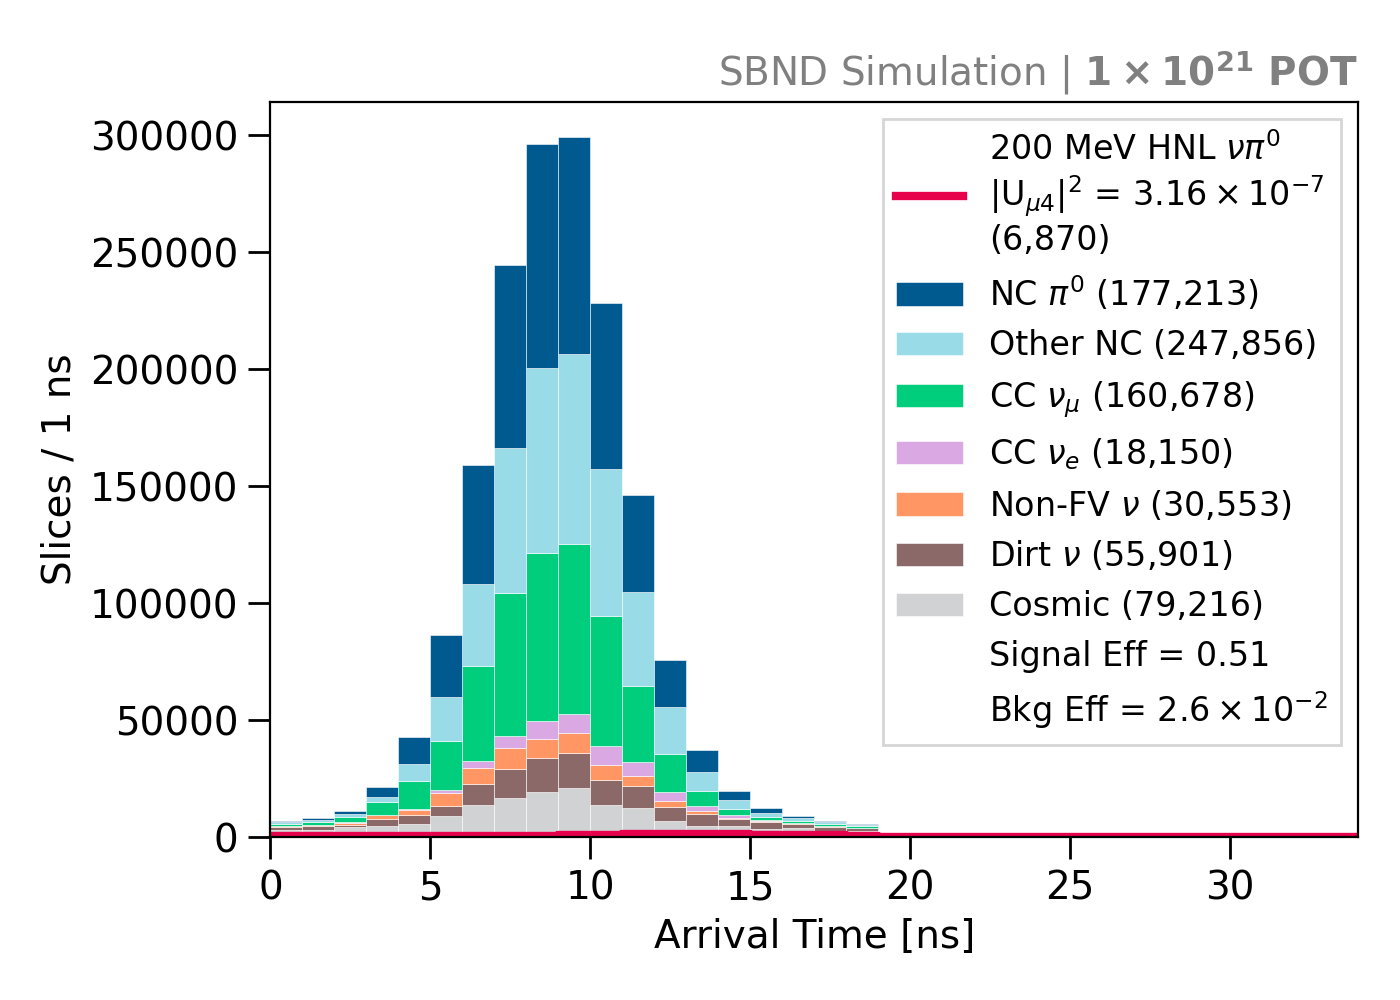
\includegraphics[width=\textwidth]{beam_bucket_postmuon}
            \caption{After muon cuts}%
            \label{fig:bb_post_muon}
        \end{subfigure}
	\caption[Muon Cuts]{
		Number of Razzled muons in a slice and Razzled muon score distributions with the cuts (top) and the arrival time distribution after the cuts (bottom). 
	}
        \label{fig:razzled_muon_cut}
\end{figure}

Similar cuts are applied consecutively to reject protons and charged pions.
As with the muon cuts, the cuts on the number of $p,\ \mu,\ \pi$ as identified by Razzled in a slice are also aggressive to require that the selected slices not contain any track-like particles.
On the other hand, the cuts on the Razzled $p,\ \mu,\ \pi$ scores were optimised for each particle type to maximise the background rejection without costing the signal efficiency.
Additional conditions are required on the reconstructed Kinetic Energy (KE) to be $ > 32.7$ MeV for protons and $< 32.1$ MeV for charged pions to ensure particles are well-reconstructed. 
The energy requirements were found to identify protons and charged pions more effectively.

The cuts to reject protons are illustrated in Fig. \ref{fig:nrazzled_proton_full} and \ref{fig:razzled_proton_score_full}.
The impacts of the proton cut can be seen in the arrival time distribution in Fig. \ref{fig:bb_post_proton}, as any interactions producing protons are removed, significantly reducing SM neutrino backgrounds.
The most impacted interaction modes are Other NC interactions reducing from $\sim249,000$ to $\sim17,000$ slices, CC $\nu_\mu$ interactions reducing from $\sim161,000$ to $\sim46,000$ slices and NC $\pi^0$ interactions reducing from $\sim 177,000$ to $\sim88,000$ slices.

The pion cuts are depicted in Fig. \ref{fig:nrazzled_pion_full} and \ref{fig:razzled_proton_score_full}. 
The result of the pion cut can be observed in the arrival time distribution shown in Fig. \ref{fig:bb_post_pion}, where the cut further cleans up any SM neutrino slices that are not already rejected by the muon and proton cuts.  
CC $\nu_\mu$ interactions are the most affected, decreasing from $\sim46,000$ to $\sim30,000$ slices.
This is followed by a reduction of Other NC interactions reducing from $\sim17,000$ to $\sim9,000$ slices.

To summarise, the cuts to reject muons, protons and charged pions are as follows:
\begin{enumerate}
\item Muon cuts:
    \begin{coloritemize}
        \item Number of Razzled-identified muons in a slice = 0,
        \item Slices containing only particles with Razzled muon score $<$ 0.04.
    \end{coloritemize}
\item Proton cuts:
    \begin{coloritemize}
        \item Number of Razzled-identified protons with KE $>$ 32.7 MeV in a slice = 0,
        \item Slices containing only particles with Razzled proton score $<$ 0.96.
    \end{coloritemize}
\item Pion cuts:
    \begin{coloritemize}
        \item Number of Razzled-identified pions KE $>$ 32.1 MeV in a slice = 0,
        \item Slices containing only particles with Razzled pion score $<$ 0.82.
    \end{coloritemize}
\end{enumerate}
The background efficiency at the end of the track removal significantly decreases by two orders of magnitudes from $\mathcal{O}(10^{-1})$ to $\mathcal{O}(10^{-3})$, demonstrating the effectiveness of these cuts.
Meanwhile, the HNL signal efficiency only decreases by 65\% to 46\%.

\begin{figure}[ht!]
        \begin{subfigure}[b]{0.495\textwidth}   
            \centering 
            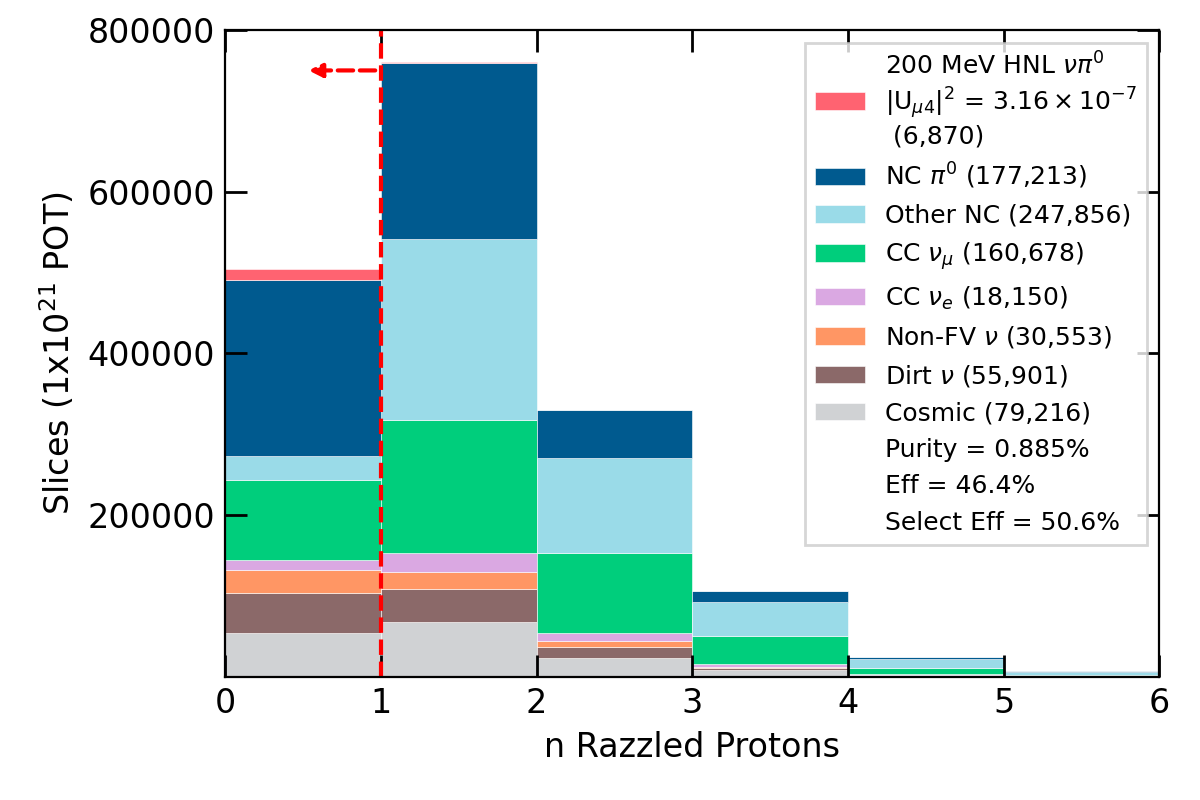
\includegraphics[width=\textwidth]{nrazzled_proton_precut}
            \caption{Number of Razzled-identified protons cut}%
            \label{fig:nrazzled_proton_full}
        \end{subfigure}
        \hfill
        \begin{subfigure}[b]{0.495\textwidth}   
            \centering 
            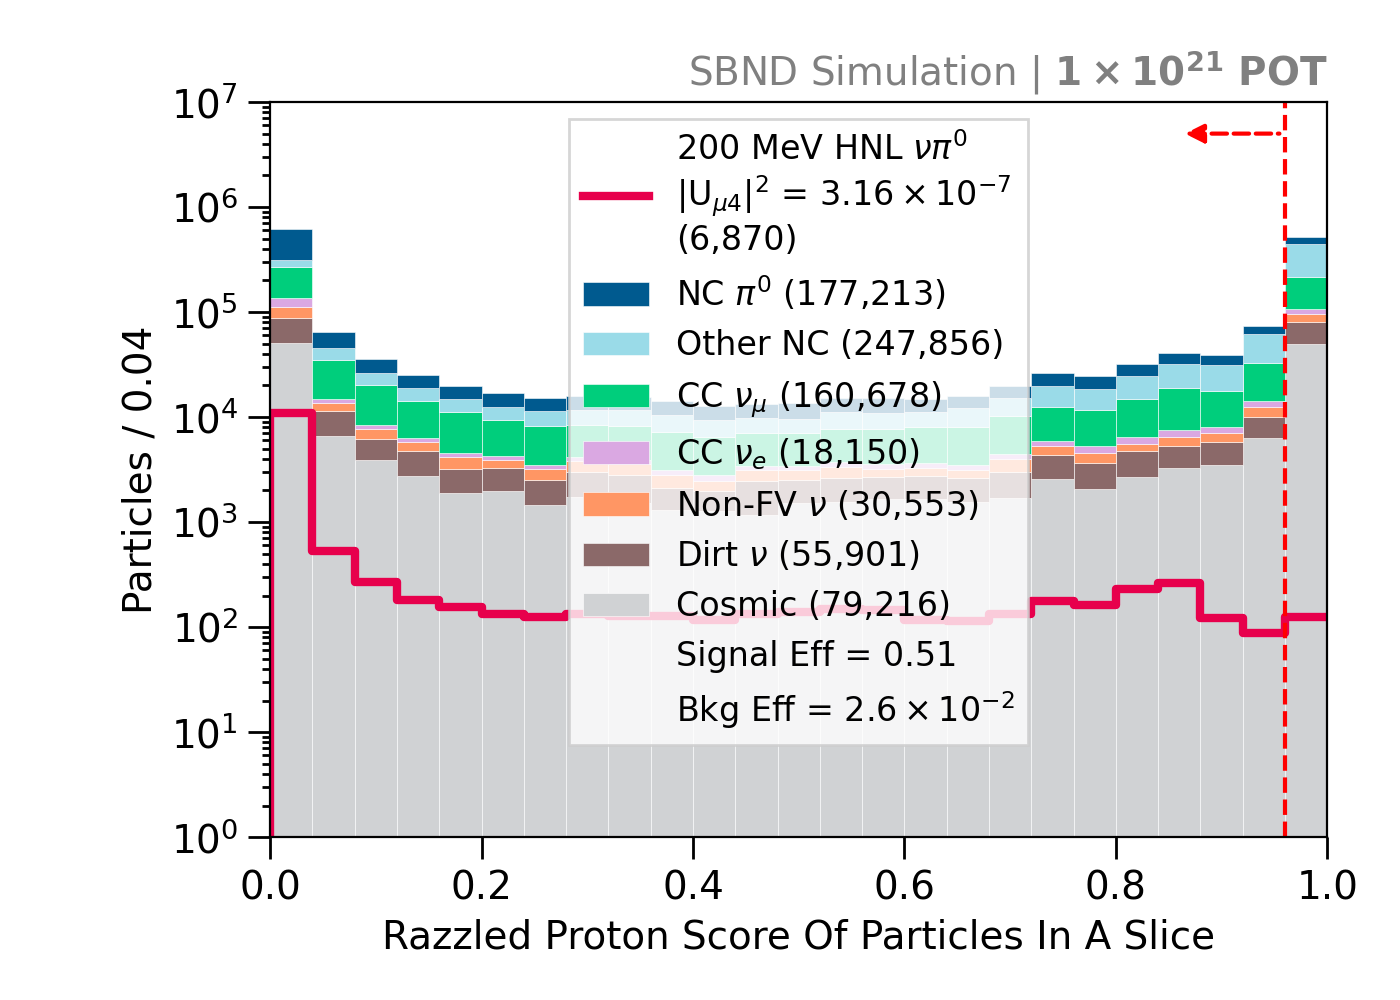
\includegraphics[width=\textwidth]{razzled_proton_score_precut}
            \caption{Particles with Razzled proton score cut}%
            \label{fig:razzled_proton_score_full}
        \end{subfigure}
        \hfill
        \begin{subfigure}[b]{0.495\textwidth}   
            \centering 
            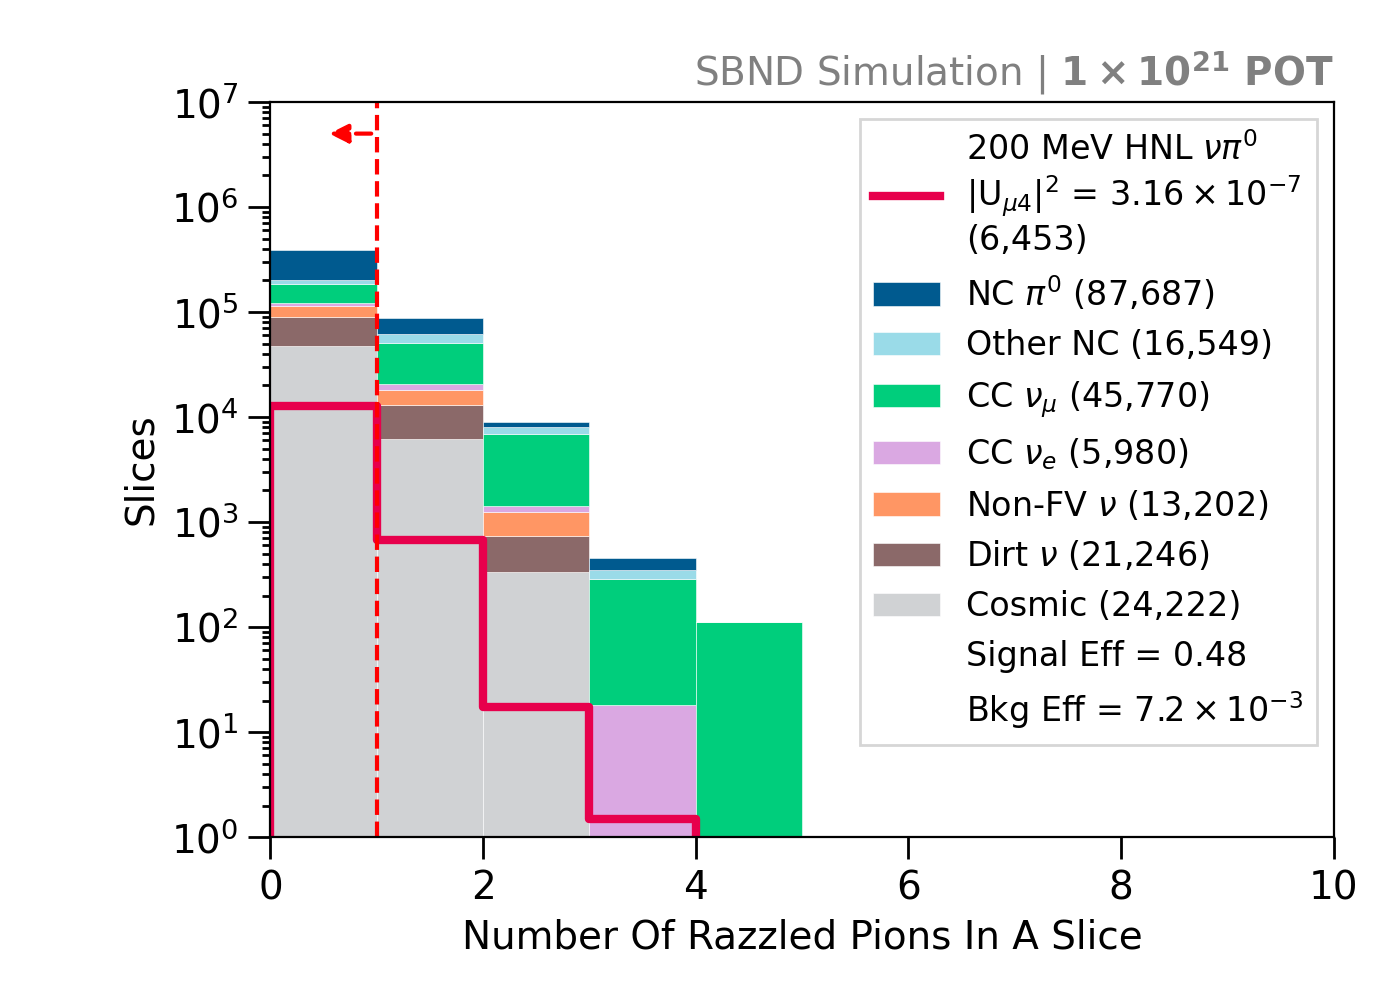
\includegraphics[width=\textwidth]{nrazzled_pion_precut}
            \caption{Number of Razzled-identified pions cut}%
            \label{fig:nrazzled_pion_full}
        \end{subfigure}
        \hfill
        \begin{subfigure}[b]{0.495\textwidth}   
            \centering 
            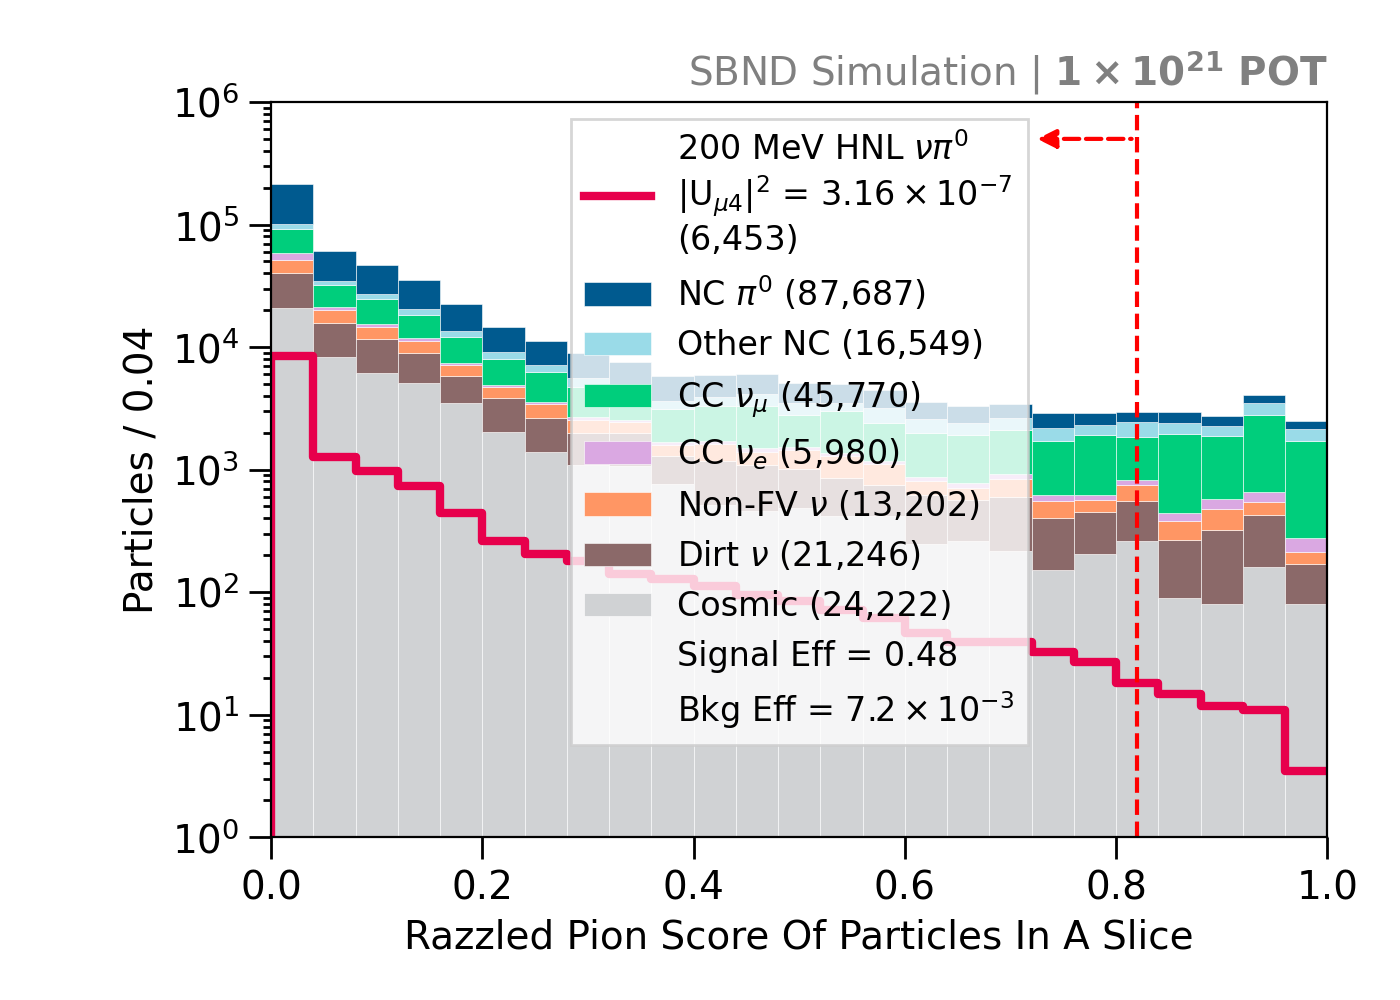
\includegraphics[width=\textwidth]{razzled_pion_score_precut}
            \caption{Particles with Razzled pion score cut}%
            \label{fig:razzled_pion_score_full}
        \end{subfigure}
	\hfill
        \begin{subfigure}[b]{0.495\textwidth}   
            \centering 
            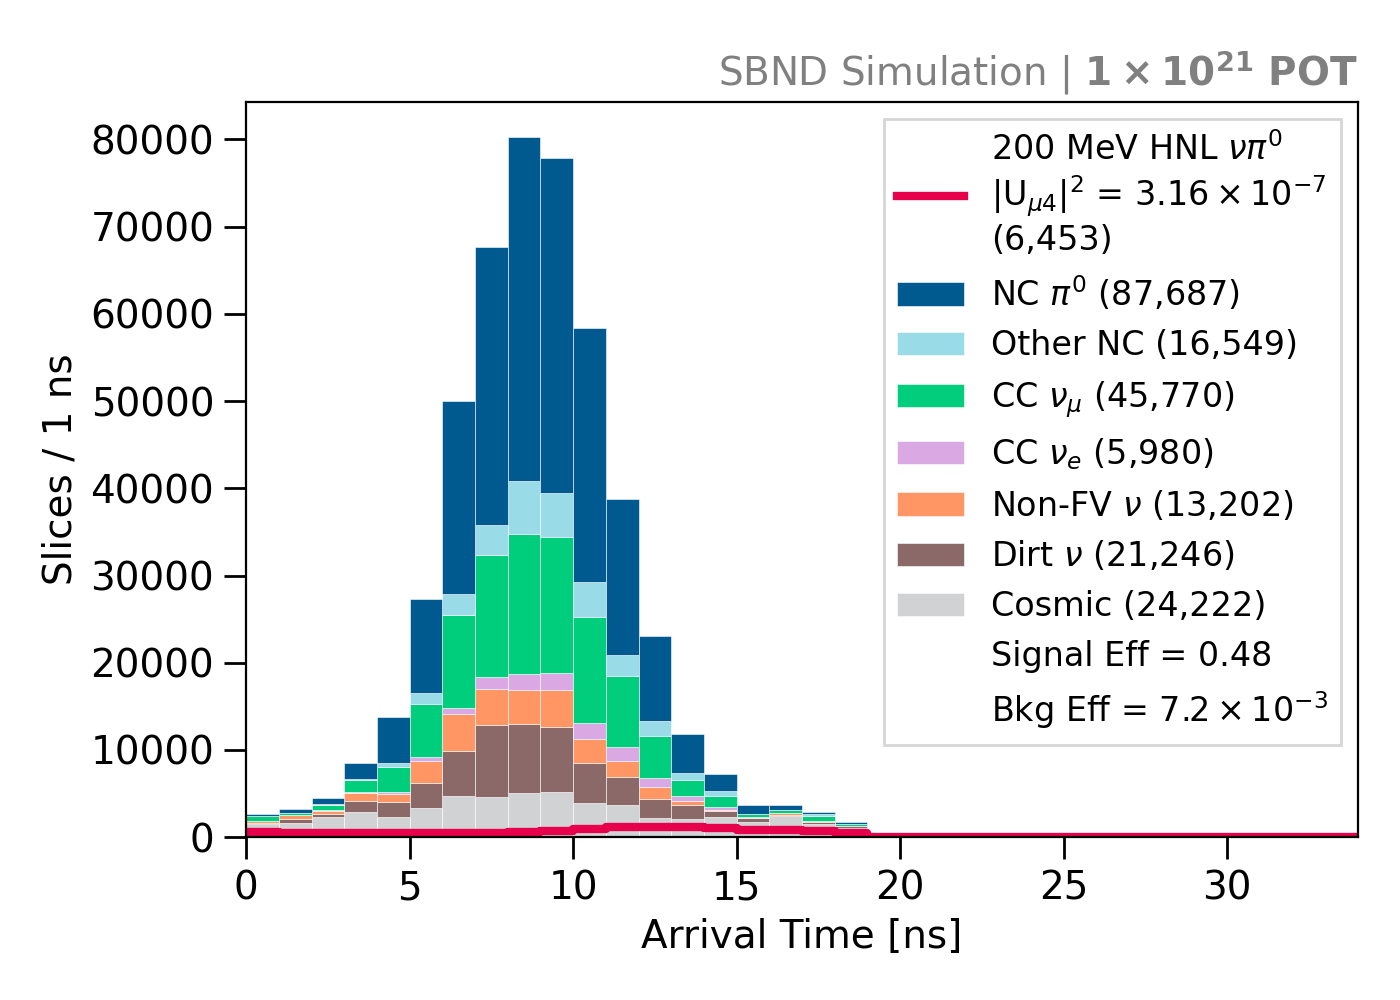
\includegraphics[width=\textwidth]{beam_bucket_postproton}
            \caption{After proton cuts}%
            \label{fig:bb_post_proton}
        \end{subfigure}
        \hfill
        \begin{subfigure}[b]{0.495\textwidth}   
            \centering 
            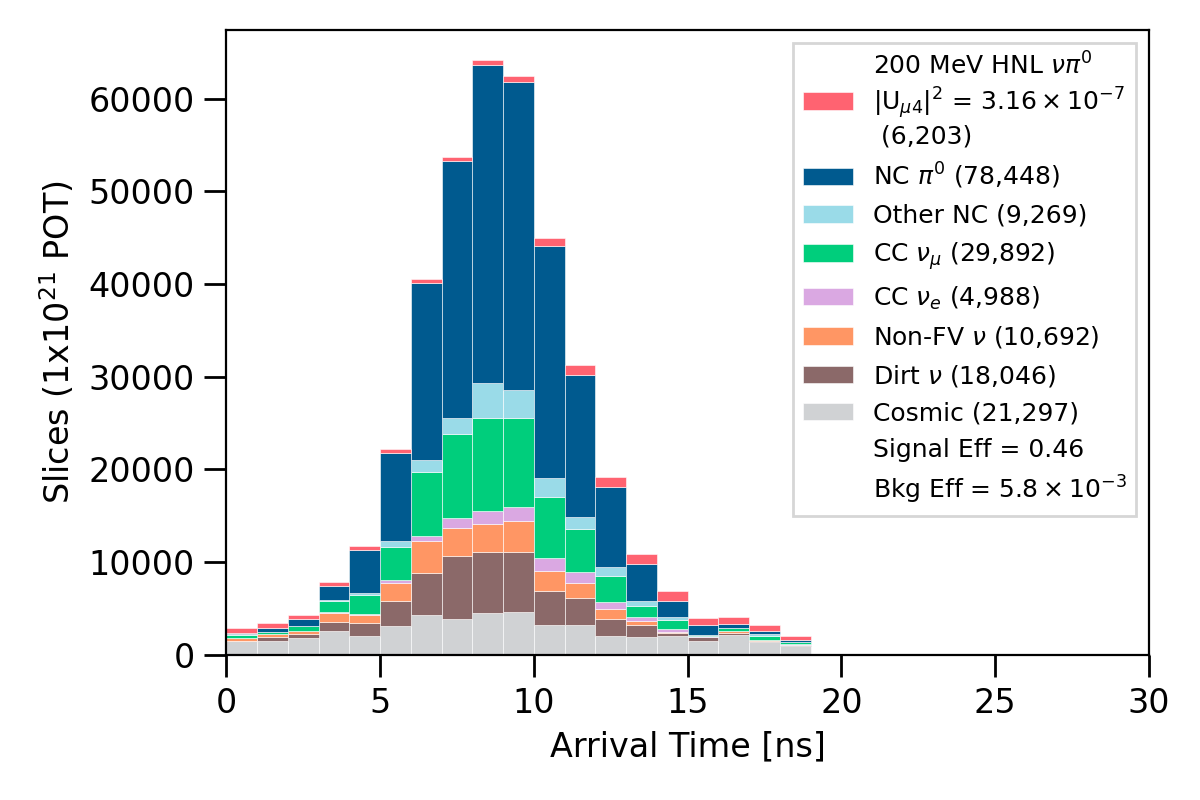
\includegraphics[width=\textwidth]{beam_bucket_postpion}
            \caption{After pion cuts}%
            \label{fig:bb_post_pion}
        \end{subfigure}
	\caption[Proton and Pion Cuts]{
		Number of Razzled protons (pions) in a slice and Razzled proton (pion) score distributions with the cuts shown at the top (middle)
		and the arrival time distribution after the proton (pion) shown at the bottom left (bottom right). 
	}
        \label{fig:razzled_proton_cut}
        %\caption{
	%	Pion cuts (top) and the arrival time after the cuts (bottom). 
	%}
        %\label{fig:razzled_pion_cut}
\end{figure}
%********************************** %First Section  **************************************
\section{Heavy Neutral Lepton Shower Selection}
\label{sec:hnl_shower_select}

After the track removal, the next five cuts target at identifying HNL showers from shower-like backgrounds.
The electron shower cut is provided in Section \ref{sec:electron_removal}.
The track score cut, to keep only very shower-like signals, is detailed in Section \ref{sec:trk_score}.
The calorimetry and theta cuts in Sections \ref{sec:calo_cut} and \ref{sec:theta_cut} exploit the boosted topology of HNL showers.
Finally, the cut on the $\pi^0$ invariant mass is given in Section \ref{sec:mass_cut}.

\subsection{Electron Shower Removal}
\label{sec:electron_removal}

%The resulting arrival time distribution after the track removal can be seen in Fig. \ref{fig:bb_post_pion}, likely contains only interactions producing showers at this stage.
%The first dominated background is from NC $\pi^0$ interactions producing di-photon showers.
%%TODO: check this statement
%This is followed by CC $\nu_\mu$ interactions likely by deep inelastic scattering producing shower-like daughter particles.
%Another dominated background is from Non-FV and dirt neutrino combined, likely by the same interaction modes with daughter products propagate and deposit energy inside the detector.

The first cut of the HNL shower selection aims at rejecting showers originating from electrons.
Key differences between electron showers and photon showers are the conversion gap and $dE/dx$ (See Section \ref{sec3:bethebloch}).
The conversion gap describes the gap between the interaction vertex and the start of the shower, where electron showers start immediately at the vertex but photon showers might propagate away from the vertex before showering. 
The $dE/dx$ describes the energy loss distribution per unit length, such that the $dE/dx$ of a photon shower is twice that of an electron shower since a photon shower is from pair production.
Both these shower characteristics are provided during the training of the Razzled BDT for classifying photons and electrons. 

\begin{figure}[b!]
        \begin{subfigure}[b]{0.495\textwidth}   
            \centering 
            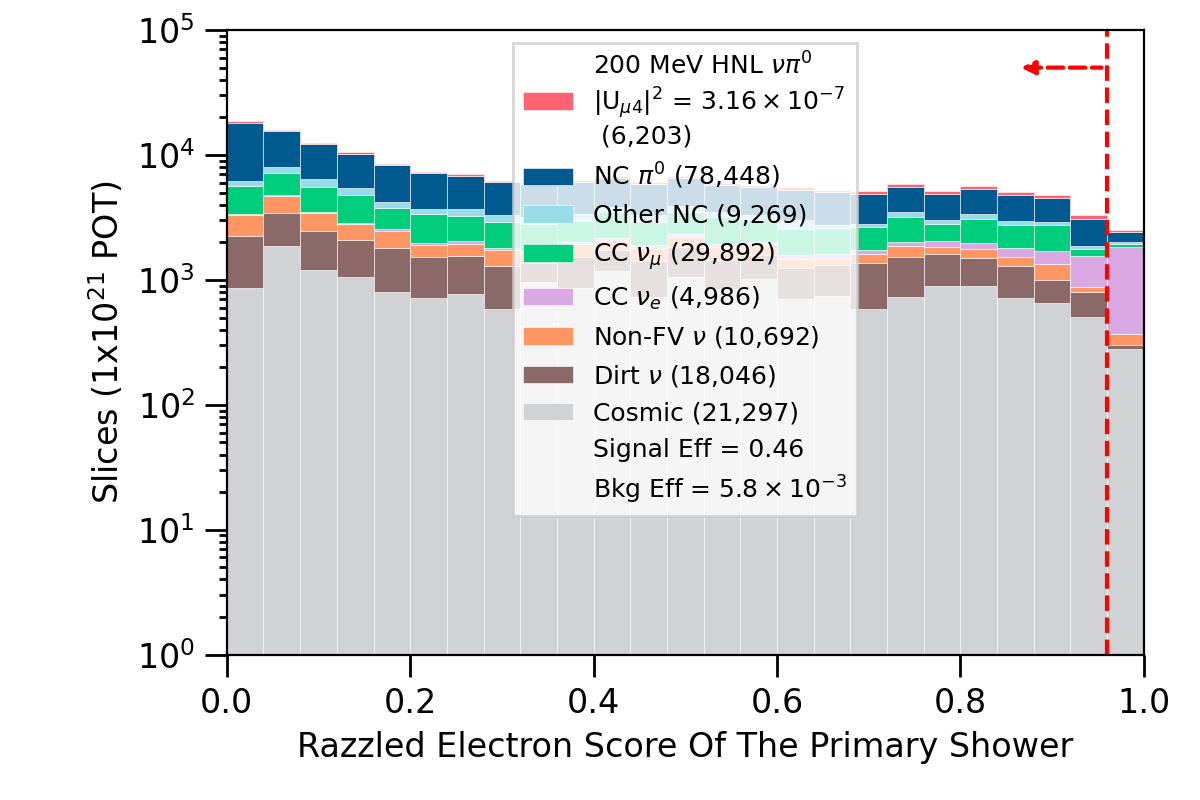
\includegraphics[width=\textwidth]{razzled_electron_score_prim_shw_precut}
            \caption{Primaries with Razzled electron score cut}%
            \label{fig:nrazzled_electron_full}
        \end{subfigure}
        \hfill
        \begin{subfigure}[b]{0.495\textwidth}   
            \centering 
            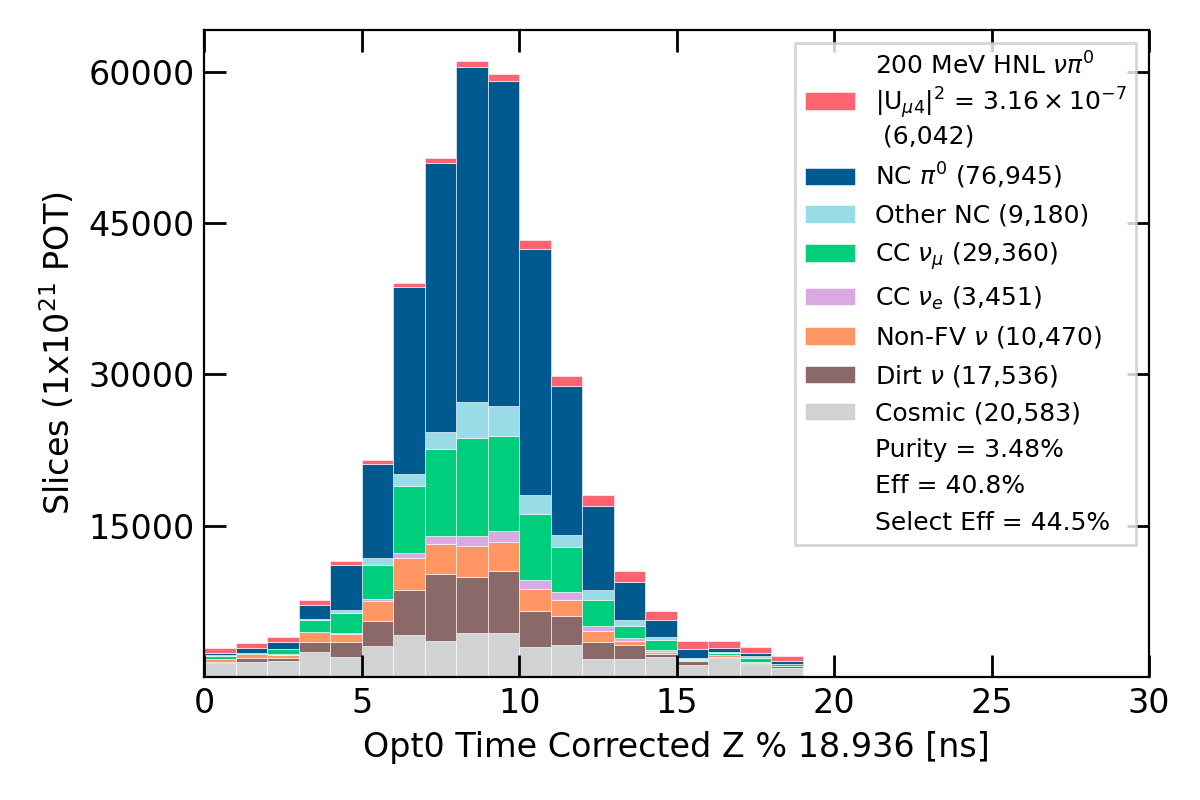
\includegraphics[width=\textwidth]{beam_bucket_postelectron}
            \caption{After electron cut}%
            \label{fig:bb_post_electron}
        \end{subfigure}
	\caption[Electron Cut]{
		Razzled electron score of the primary shower distribution with the cut (left) and the arrival time distribution after the cut (right). 
	}
        \label{fig:razzled_electron_cut}
\end{figure}

The Razzled electron score is examined for the primary shower that deposits the most energy in a slice.
The cut is demonstrated in Fig. \ref{fig:razzled_electron_cut}, where only slices containing primary showers with a Razzled electron score $< 0.96$.
The rejected slices are clearly-identified CC $\nu_e$ showers with high Razzled electron scores.
This is a very soft cut compared to the previous track removal cuts since showers from CC $\nu_e$ interactions and showers from HNLs are very similar to each other.
The cut rejects $31\%$ of the remaining $\sim5,000$ CC $\nu_e$ slices while minimally reduces HNL slices by only $3 \%$.

%********************************** %First Section  **************************************
\subsection{Track Score Cut}
\label{sec:trk_score}

%The next set of cut after SM neutrinos removal focus on identifying HNL showers from the trickier background from SM NC $\pi^0$ interactions.
To further reject backgrounds containing showers, careful considerations were taken into developing cuts by separating the shower topology into subsets.
As previously stated, di-photon showers from HNLs can result in either a single shower topology or multiple shower topology.
Thus, two cases can be considered when applying cuts: (1) slices containing only one shower and (2) slices containing two or more showers.
The distribution of signal and background slices in the phase space of the cut variable vary differently between the two cases.
This results in a different signal-to-background ratio across the distribution for each case.
From this cut onwards, individual cut is examined per case to optimise the efficiency of background rejection and signal selection. 

\begin{figure}[ht!]
        \begin{subfigure}[b]{0.495\textwidth}   
            \centering 
            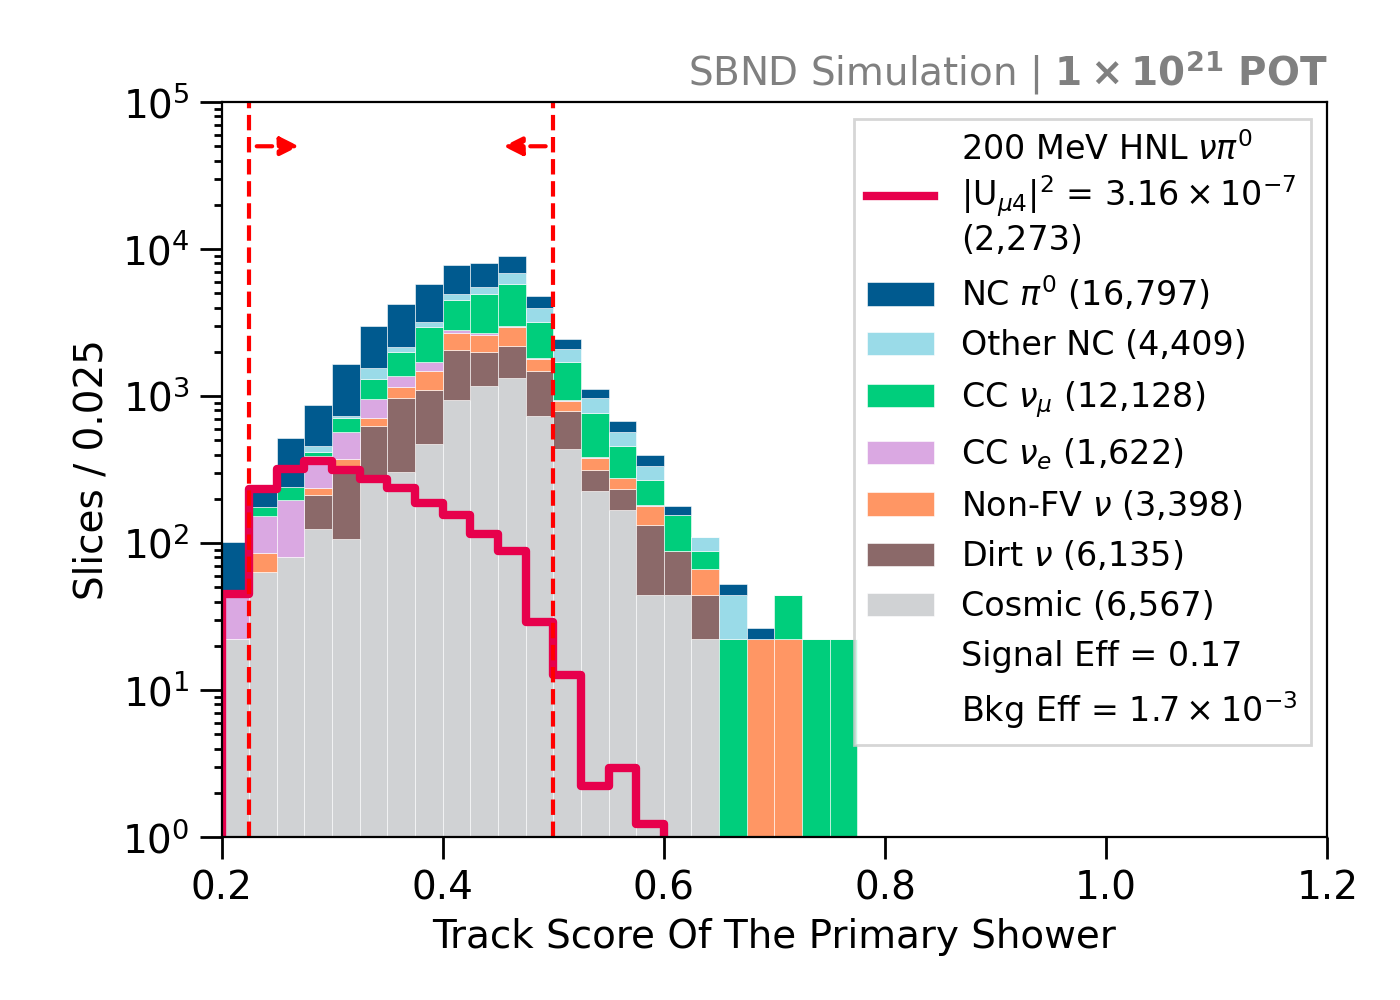
\includegraphics[width=\textwidth]{one_shw_track_score}
            \caption{1 Shower Case: Track score cut}%
        \end{subfigure}
        \hfill
        \begin{subfigure}[b]{0.495\textwidth}   
            \centering 
            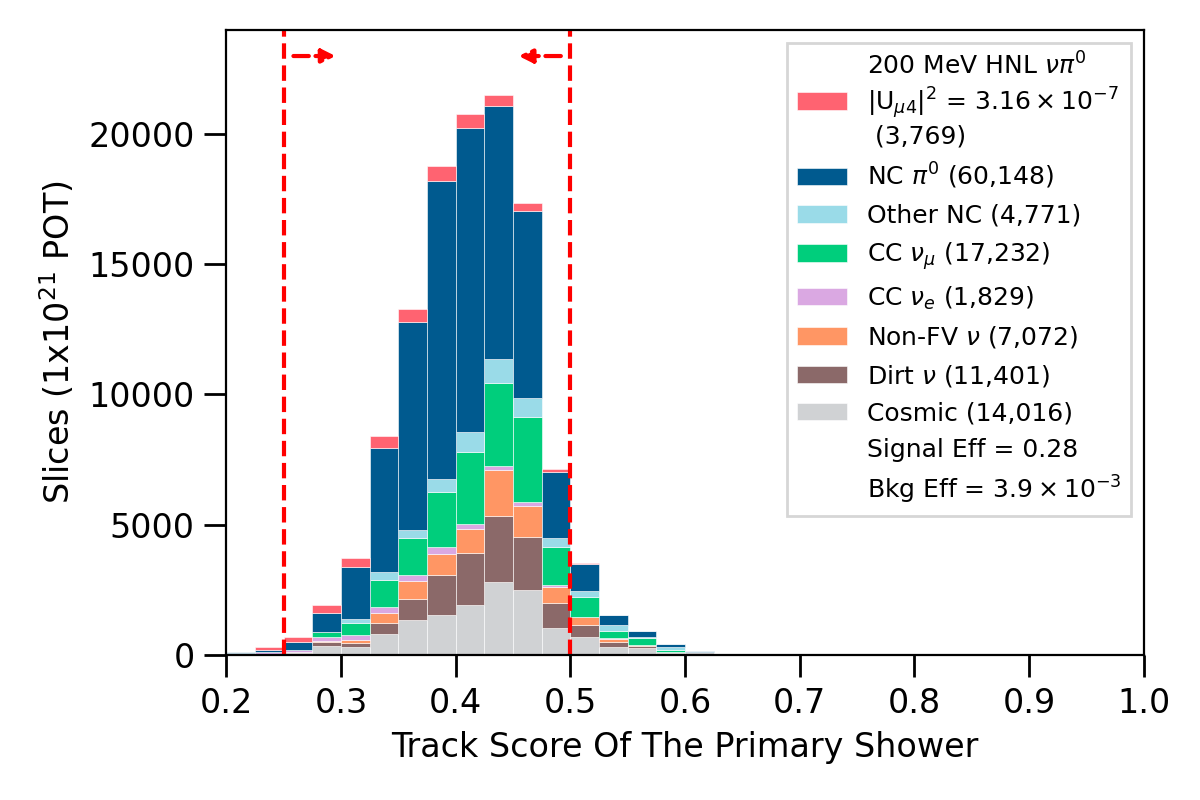
\includegraphics[width=\textwidth]{two_shower_primary_track_score_precut}
            \caption{2+ Showers Case: Track score cut}%
        \end{subfigure}
        \hfill
	\centering
        \begin{subfigure}[b]{0.495\textwidth}   
            \centering 
            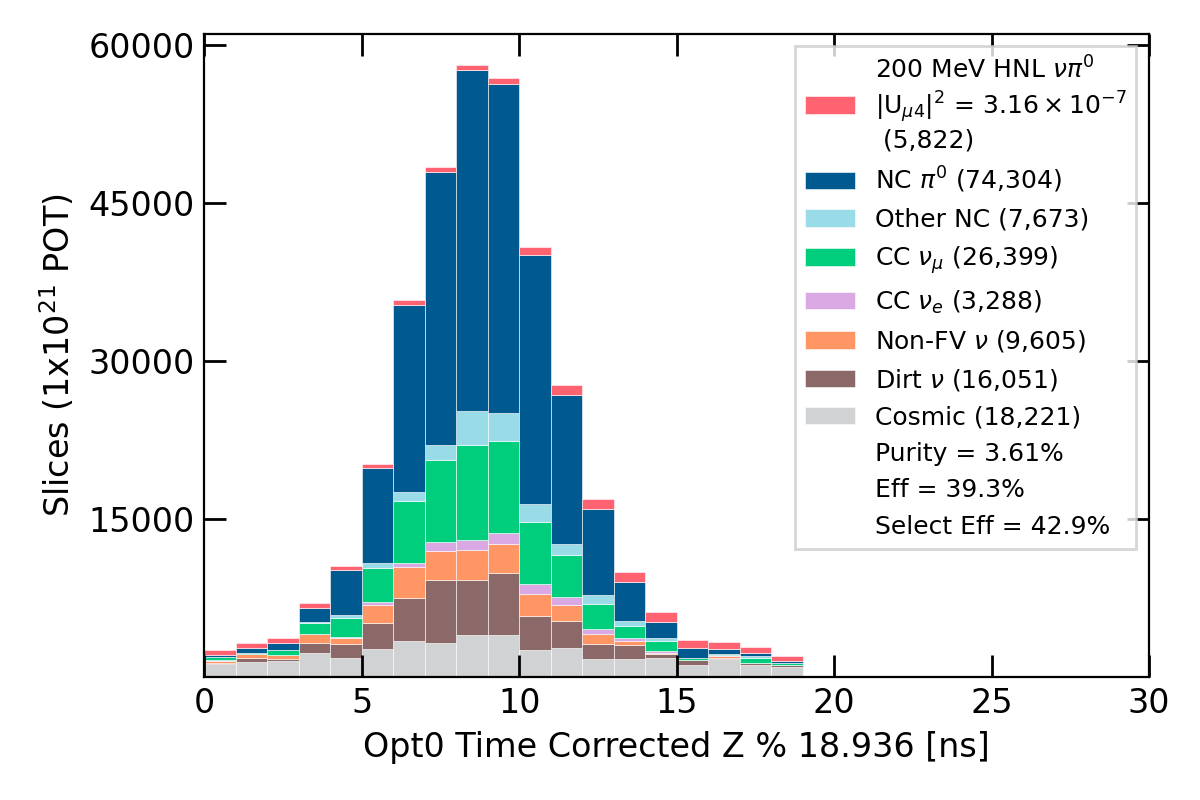
\includegraphics[width=\textwidth]{beam_bucket_postrackscore}
            \caption{After track score cut}%
	    \label{fig:bb_track_score}
        \end{subfigure}
	\caption[Track Score Cut]{
		Track score distributions with the cuts (top) and the arrival time distribution after the cut (bottom). 
	}
        \label{fig:track_score_cut}
\end{figure}

The second cut of the HNL shower selection employs the track-shower separation BDT, that outputs a track score to a particle indicating if it is track-like or shower-like (See Section \ref{sec:trkshwbdt}).
The track score is  examined for the primary shower that deposits the most energy in a slice.  
Fig. \ref{fig:track_score_cut} displays the track score distribution of primary particles for the two cases of slices containing 1 shower and 2+ showers.
For both cases, the remaining primary particles are already shower-like since the track score concentrates at $< 0.5$.

%ratio is higher across the score distribution the single shower case than the multiple showers case.
The cut sets the upper boundary of the track score at 0.5 for both cases, to reject any primary particles leaning towards track-like.
On the other hand, the cut on the lower boundary of track score aims at trimming some shower-like backgrounds.
The cut is optimised for each case depending on its signal-to-background distribution.
A more lenient cut is applied for the single shower case selecting primary showers with a track score of $\geq 0.225$.
The cut is tightened up for the multiple showers case for better background rejection, requiring primary showers to have a track score of $\geq 0.25$.
The resulting arrival time distribution is depicted in Fig. \ref{fig:bb_track_score}, showing a reduction of 3-16\% across different SM neutrino interaction types.
The signal selection efficiency only reduces from 45\% to 43\%.

\subsection{Calorimetry Cut}
\label{sec:calo_cut}

The third cut of the HNL shower selection targets the highly energetic aspect of HNL showers compared to SM neutrino showers.
Outputs from the slice-to-flash matching process are examined, particularly the fraction variable defined in Eq. \ref{eq:opt0fraction} in Section \ref{sec:subsystem_match}.
The fraction describes the level of agreement between $L_{\mathrm{Q}}$ and $L$, where $L_\mathrm{Q}$ is the number of PhotoElectrons (PEs) predicted from the reconstructed charge and $L$ is the number of PEs measured by PMTs.
A large disagreement indicates poor reconstruction, whether under or overestimation in between reconstructed energy from charge and light.

The fraction is useful to identify showers originated from HNLs due to their boosted topologies.
Very forward-going HNL showers are likely to overlap and reconstructed as a single shower merged from multiple showers.   
The reconstructed charge of the merged HNL shower tends to be much higher than that for SM neutrinos.
The number of PEs predicted from the reconstructed charge $L_{\mathrm{Q}}$ is therefore likely to be overestimated compared to the number of PEs measured by PMTs $L$.

\begin{figure}[bp!]
        \begin{subfigure}[b]{0.495\textwidth}   
            \centering 
            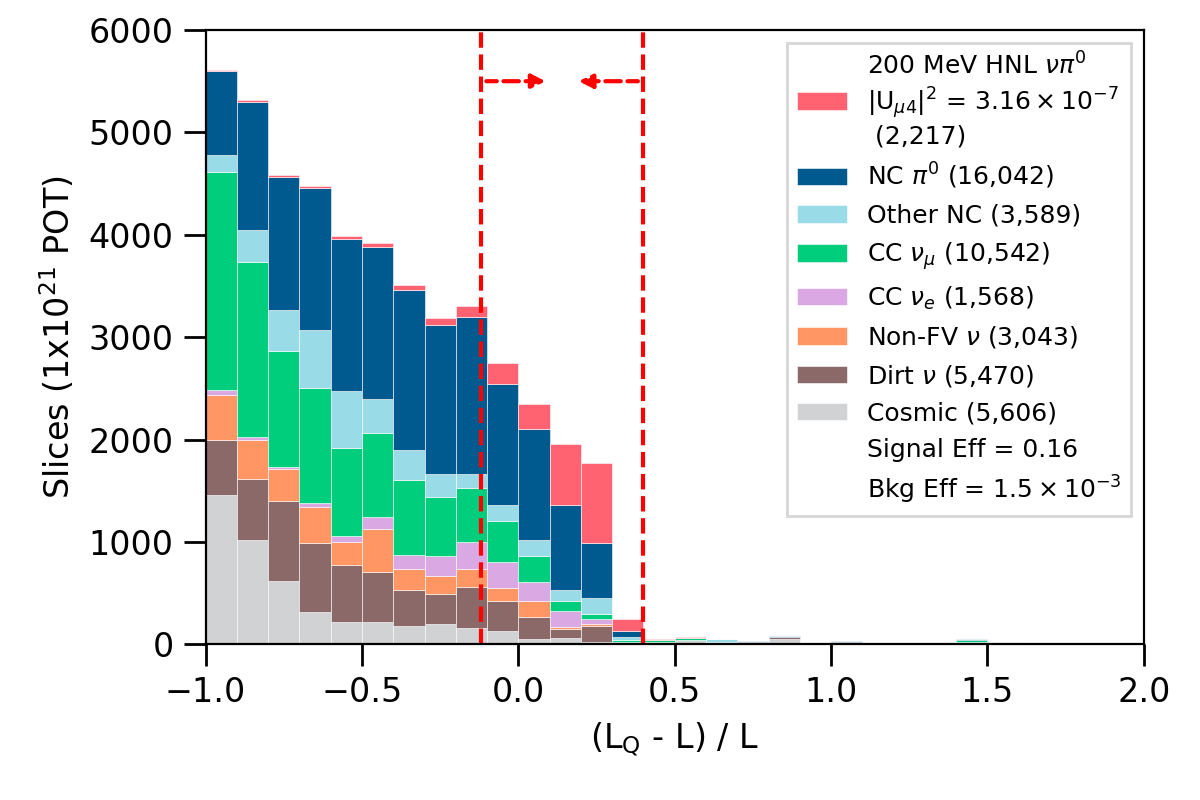
\includegraphics[width=\textwidth]{opt0frac_one_shw_precut}
            \caption{1 Shower Case: Calorimetry cut}%
        \end{subfigure}
        \hfill
        \begin{subfigure}[b]{0.495\textwidth}   
            \centering 
            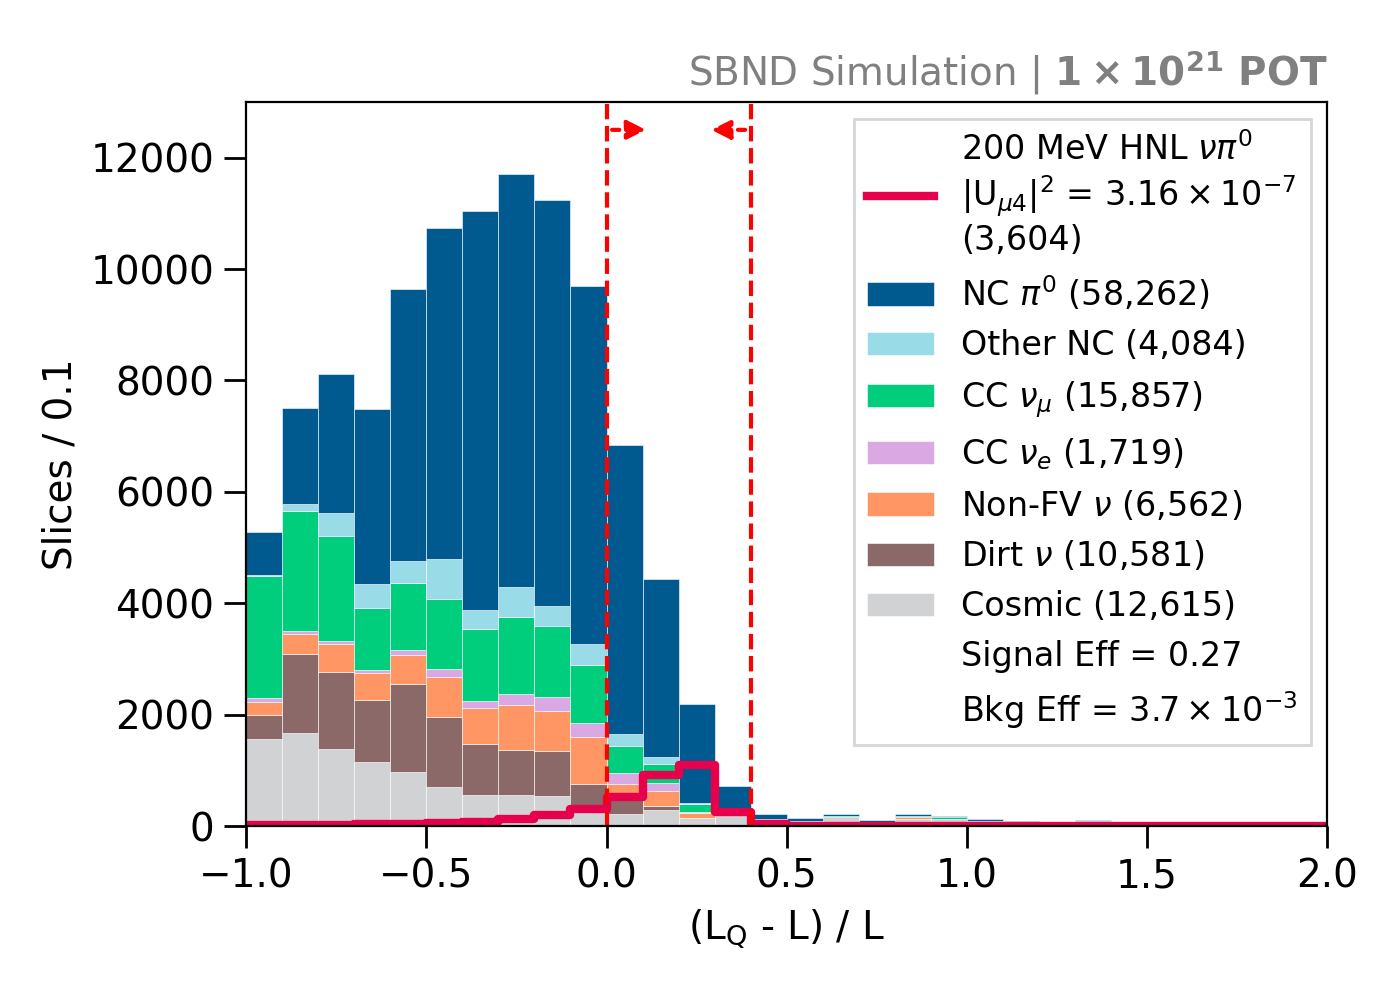
\includegraphics[width=\textwidth]{opt0frac_two_shw_precut}
            \caption{2+ Showers Case: Calorimetry cut}%
        \end{subfigure}
        \hfill
	\centering
        \begin{subfigure}[b]{0.495\textwidth}   
            \centering 
            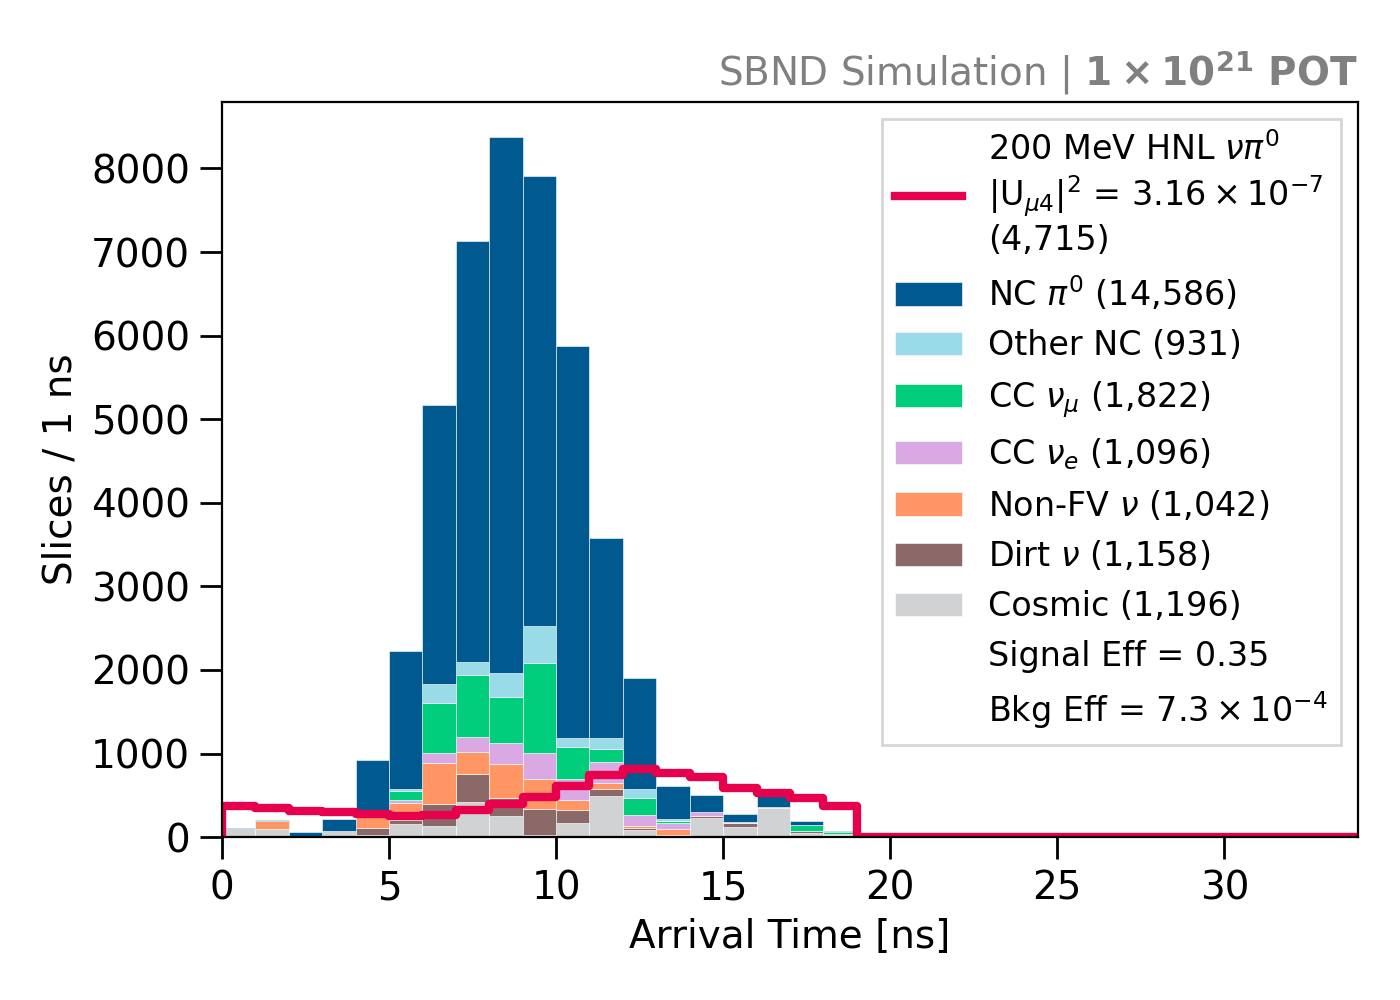
\includegraphics[width=\textwidth]{beam_bucket_postopt0}
            \caption{After Calorimetry cut}%
	    \label{fig:bb_opt0}
        \end{subfigure}
	\caption[Calorimetry Cut]{
	Distributions of the ($L_{\mathrm{Q}} - L)/L$ with the cuts (top) and the arrival time distribution after the cut (bottom). 
	}
        \label{fig:opt0_cut}
\end{figure}

The overestimation is demonstrated in Fig. \ref{fig:opt0_cut}, where it can be seen that HNL slices mainly concentrate in the region $\frac{(L_{\mathrm{Q}} - L)}{L} \geq 0$. 
The calorimetry cut exploits this feature and is optimised for the single shower as well as the multiple shower case.
For slices containing a single shower, the requirement on the fraction is between -0.1 and 0.4 to select well-predicted showers with the fraction centred around 0, as well as overestimated showers with the fraction $> 0$. 
For slices containing multiple showers, the requirement on the fraction is restricted to between 0.04 and 0.3 to select only overestimated showers, rejecting backgrounds more aggressively.
The arrival time distribution after the cut is shown in Fig. \ref{fig:bb_opt0}, demonstrating the effectiveness of the cut as the background efficiency decreases by a whole order of magnitude from $\mathcal{O}(10^{-3})$ to $\mathcal{O}(10^{-4})$. 
Meanwhile, the signal selection efficiency only decreases from 43\% to 35\%.

\subsection{Theta Angle Cut}
\label{sec:theta_cut}

The fourth cut exploits the topology of the forward-going HNL showers such that their angles with respect to the beam direction, referred to as \textit{theta angles}, are small.
Fig. \ref{fig:1shw_theta_cut} shows the angular distribution for slices containing a single shower.
In this case, the signals are mainly highly energetic and boosted di-photon showers reconstructed as a single merged and beam-collimated shower.
As a result, their theta angles concentrate in the region $< 25^{\circ}$.
An aggressive selection of $< 25^{\circ}$ can be placed without compromising signal efficiency.
%due to the high signal-to-background ratio in this region.
\begin{figure}[bp!]
        \begin{subfigure}[b]{0.495\textwidth}   
            \centering 
            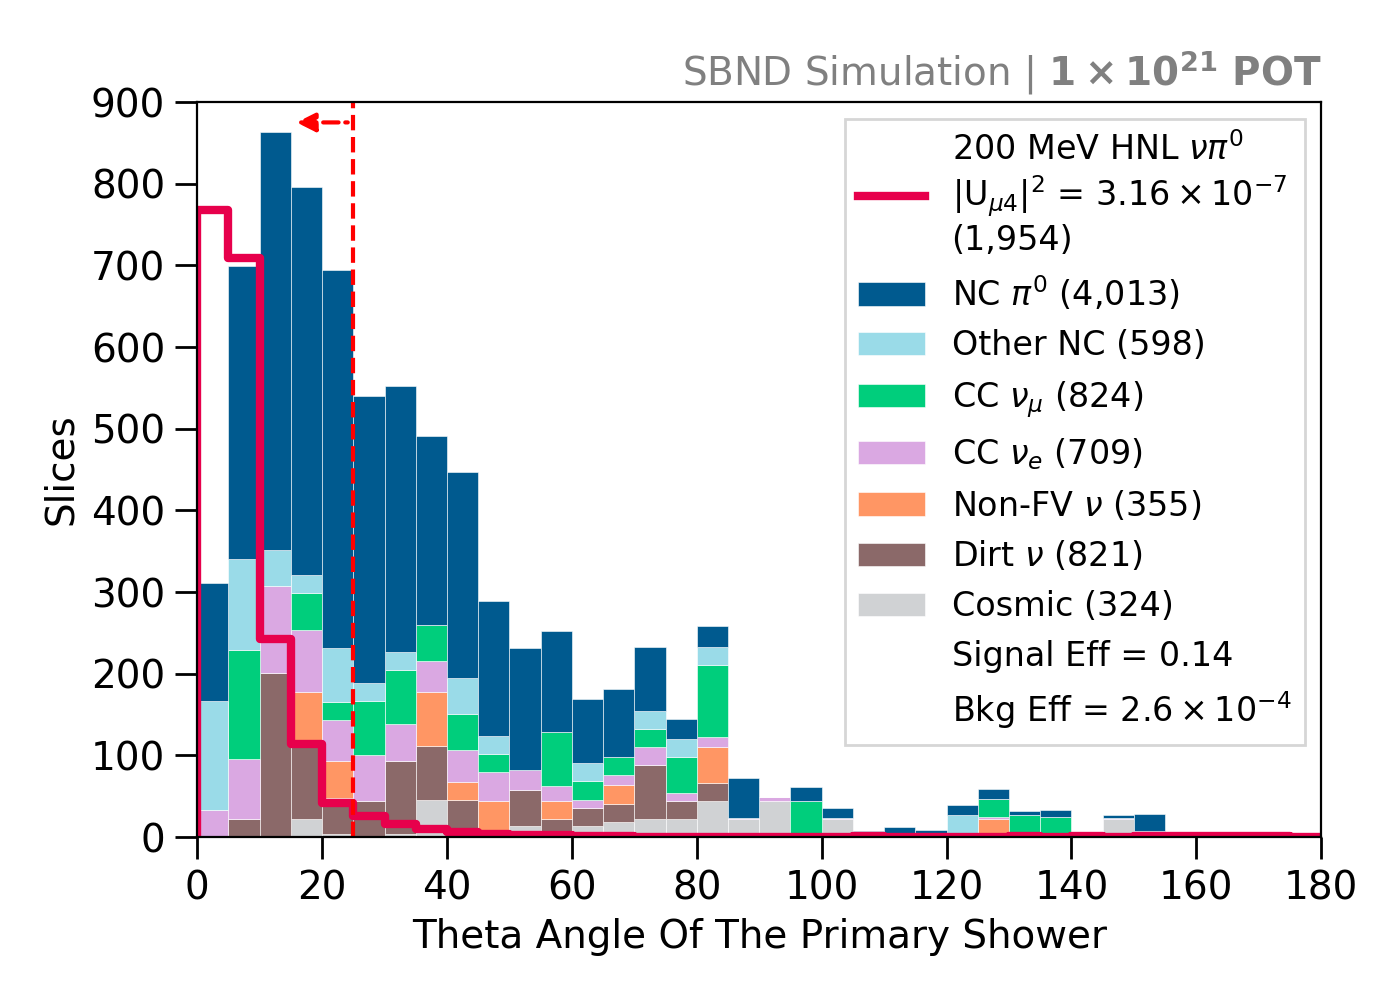
\includegraphics[width=\textwidth]{one_shower_theta_precut}
            \caption{1 Shower Case: Theta angle cut}%
	    \label{fig:1shw_theta_cut}
        \end{subfigure}
        \hfill
        \begin{subfigure}[b]{0.495\textwidth}   
            \centering 
            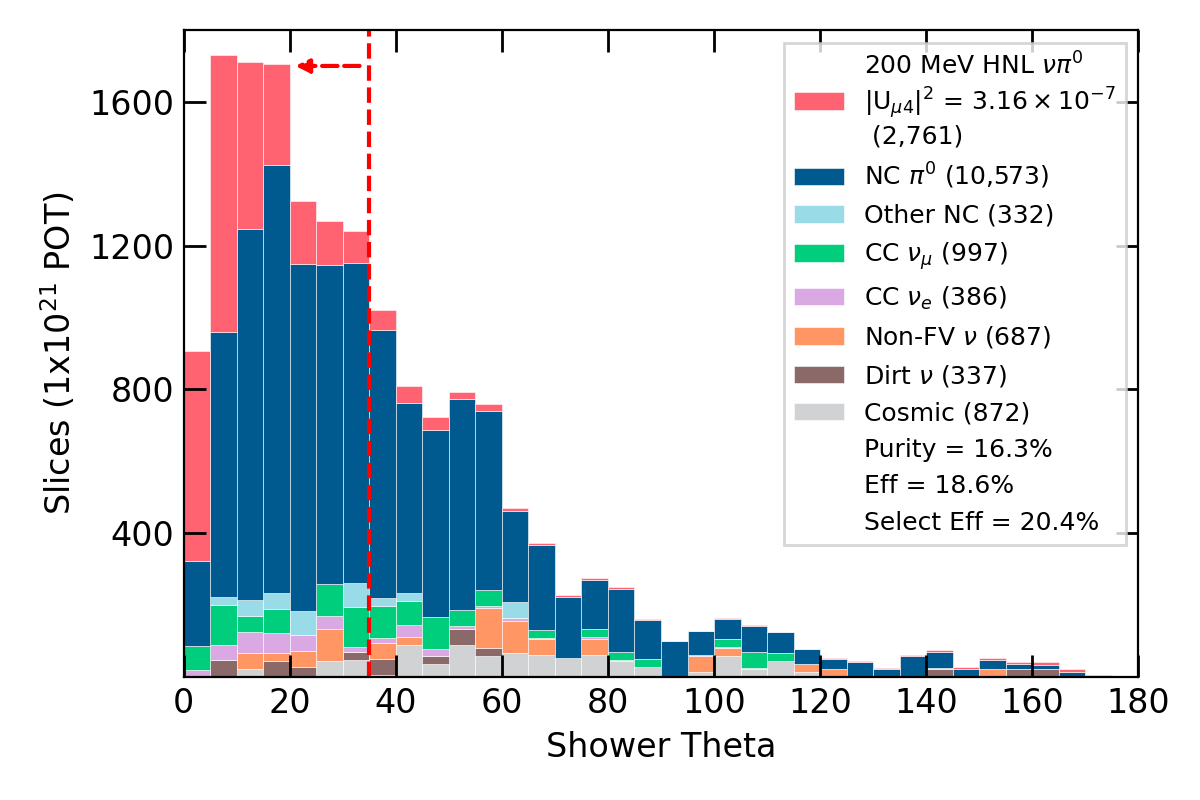
\includegraphics[width=\textwidth]{two_shower_primary_theta_precut}
            \caption{2+ Showers Case: Theta angle cut}%
	    \label{fig:2shw_theta_cut}
        \end{subfigure}
        \hfill
	\centering
        \begin{subfigure}[b]{0.495\textwidth}   
            \centering 
            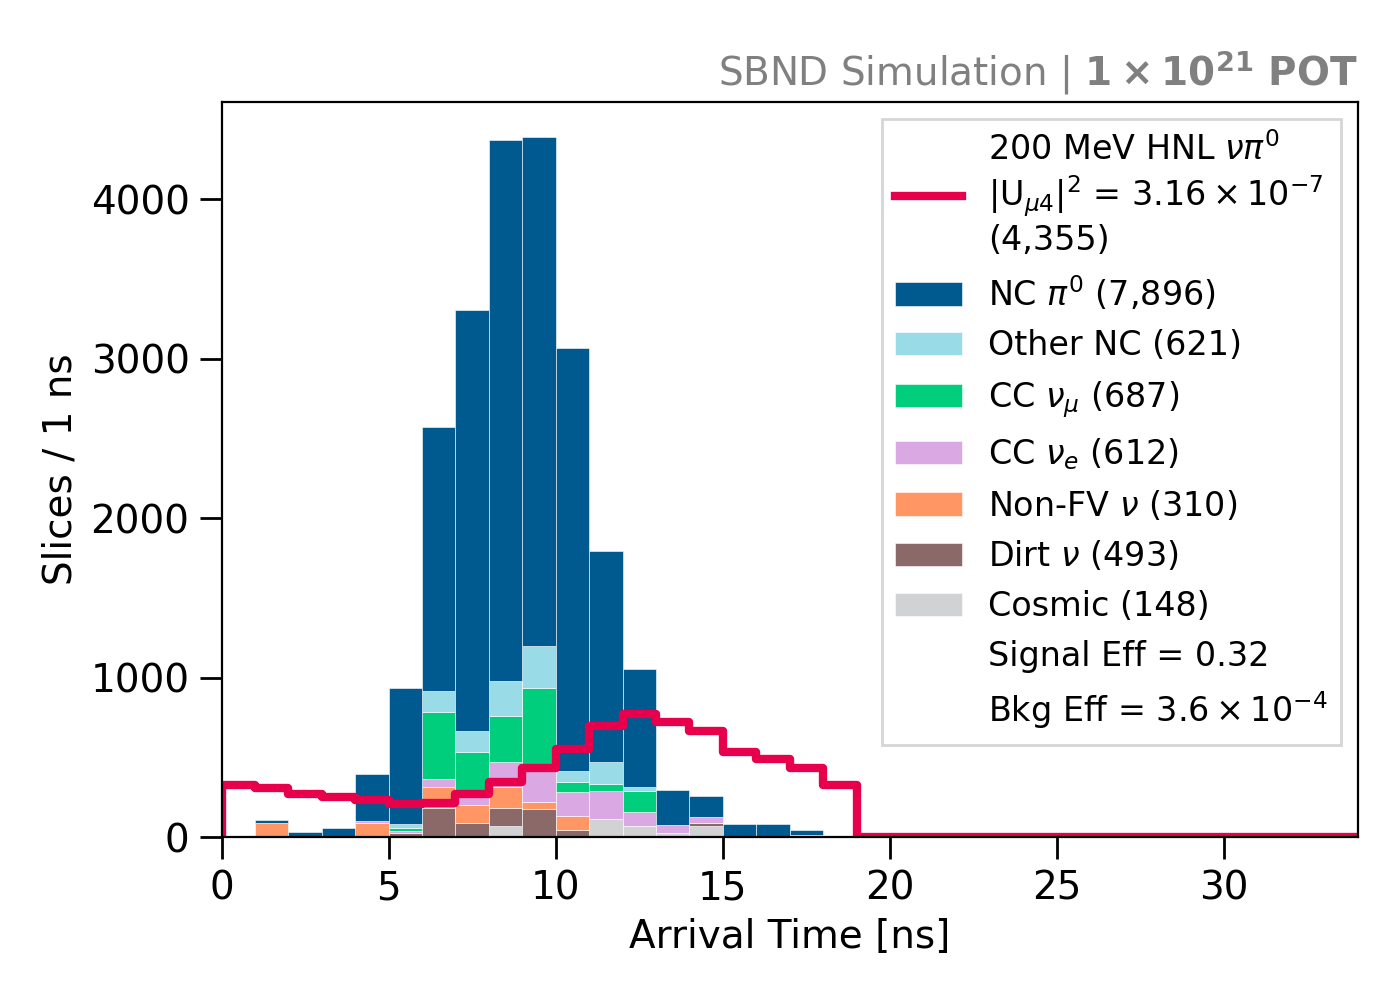
\includegraphics[width=\textwidth]{beam_bucket_postshowertheta}
            \caption{After theta angle cut}%
	    \label{fig:bb_theta}
        \end{subfigure}
	\caption[Theta Angle Cut]{
		Theta angle distributions with the cuts (top) and the arrival time distribution after the cut (bottom). 
	}
        \label{fig:theta_cut}
\end{figure}

Fig. \ref{fig:2shw_theta_cut} shows the theta angle distribution for slices containing multiple showers.
In this case, HNL showers are less boosted and more likely to result in separated showers.
Their theta angles with respect to the beam are larger compared to the single shower case.
To preserve signal selection efficiency, a widened selection of $< 30^{\circ}$ is applied.

Fig. \ref{fig:bb_theta} shows the arrival time distribution after applying the cut.
The theta angle cut effectively rejects any shower-like backgrounds that are not beam-collimated, resulting in a reduction across all SM neutrino interaction types.
This is a very impactful cut given that the background efficiency decreases by half from $7.3 \times 10^{-4}$ to $3.6 \times 10^{-4}$.
The signal efficiency of HNL slices only drops from 35\% to 32\%.

\subsection{Neutral Pion Invariant Mass Cut}
\label{sec:mass_cut}

\begin{figure}[b!]
        \centering 
        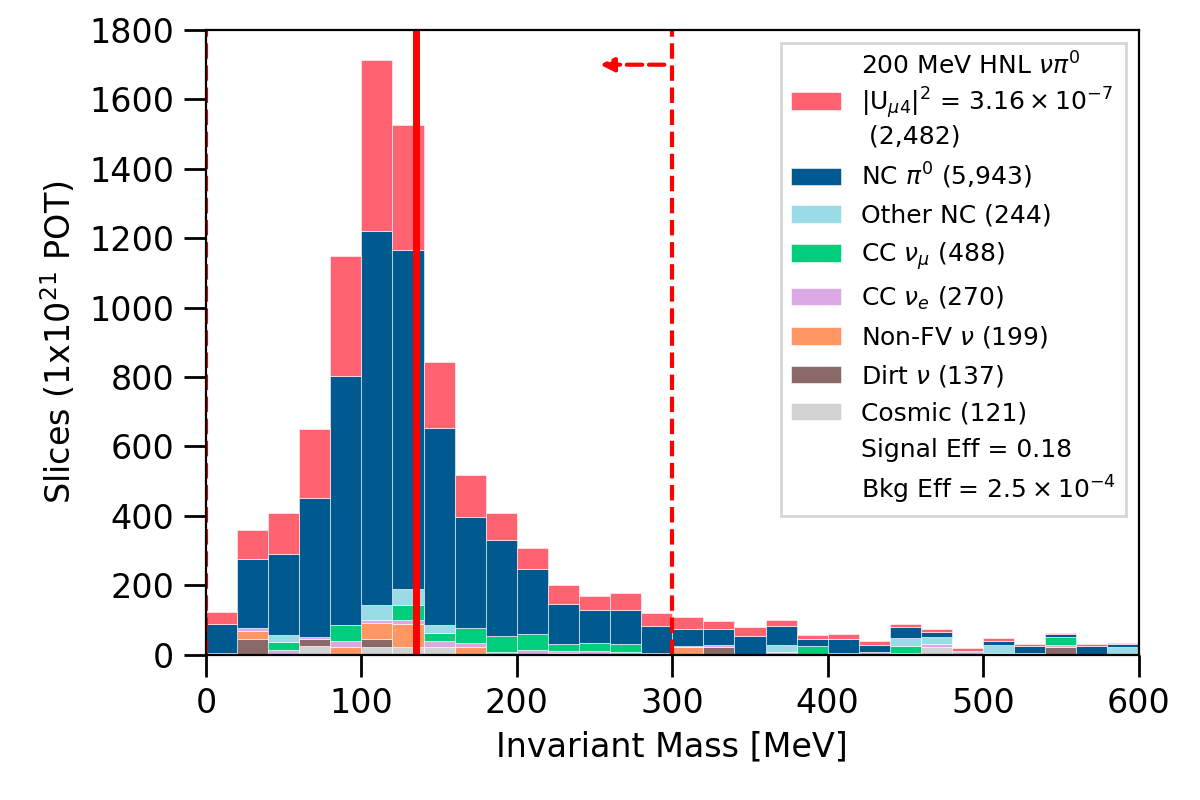
\includegraphics[width=0.495\textwidth]{pizero_mass_precut}
	\caption[Neutral Pion Invariant Mass Cut]{
	$\pi^0$ invariant mass distribution with the cut applied to the multiple showers case.
	}
        \label{fig:mass_cut}
\end{figure}

The final cut of the HNL shower selection exploits the fact that di-photon showers originate from a $\pi^0$ decay, allowing for the reconstruction of $\pi^0$ invariant mass, $m_{\pi^0}$.
For slices containing multiple showers, the invariant mass is reconstructed using the reconstructed momenta of any two shower combination in the slice.
For two massless photon showers with an opening angle $\alpha$ and a total energy $E_1$ and $E_2$ respectively, $m_{\pi^0}$ is computed as:
\begin{equation}
	m_{\pi^0} = \sqrt{2 E_1 E_2 \times (1 - \mbox{cos}\alpha)}.
\end{equation}
For a given slice, the $\pi^0$ invariant mass was reconstructed for all combinations of two showers, and the best mass was considered for the cut.
The cut is illustrated in Fig. \ref{fig:mass_cut}, where the solid red line indicates the $\pi^0$ mass of 135 MeV.
A cut is applied to select slices corresponding to a reconstructed invariant mass of 300 MeV or less.
This rejects any slices with a poorly reconstructed $\pi^0$ mass, which could be due to backgrounds from 
SM neutrino interactions such as CC $\nu_\mu$, Other NC, Non-FV and dirt as well as energetic cosmic rays.
However, poor shower reconstruction can also result in di-photon showers from $\pi^0$ getting mistakenly rejected by this cut, as it is evident that some NC $\pi^0$ interactions and HNL signals are affected.
This cut reduces both signal and background slices by $< 3 \%$.


\section{Selection Results}
\label{sec:select_result}

Fig. \ref{fig:bb_full_loose} shows the arrival time distribution after the selection.
The background efficiency is $3.3 \times 10^{-4}$, demonstrating the extreme background rejection achieved amounting to four orders of magnitude.
Meanwhile, the signal efficiency is well-preserved at $30\%$. 
The remaining background is dominated by NC $\pi^0$ interactions, which are tricky to remove due to their similarities with HNLs.
A combination of CC $\nu_\mu$ and Other NC interactions remain, likely undergo deep inelastic scattering, producing shower-like products like $\pi^0$ or $e^{\pm}$.
CC $\nu_e$ interactions persist as they can produce a single shower topology. 
Some Non-FV and dirt neutrino interactions can still be seen, since their products can propagate to the FV and deposit energy.  
Finally, cosmic muons are almost fully rejected. 

The multi-binned analysis for determining sensitivity depends on signal-rich bins.
Fig. \ref{fig:bb_edge_loose} zooms into the first and last 4 bins of the arrival time distribution, which are the highest the signal-to-background ratio bins.
These contribute towards sensitivity significantly more than bins located at the centre region of the distribution. 
A \textit{timing cut} can be applied to select only these bins, which would result in a background efficiency decreasing from $\mathcal{O}(10^{-4})$ to $\mathcal{O}(10^{-6})$ while still maintain a signal efficiency of 10\%.
However, the cut is not formally applied as part of the selection, but to highlight the importance of these edge bins due to their excellent signal-to-background ratio.
The timing cut is discussed further in Chapter \ref{ChapterResult}.

To better understand the sensitivity dependence on the signal-to-background ratio, two selections were developed.
The selection presented up until this point is referred to as \textit{the lenient cut}.
An additional more aggressive cut, referred to as \textit{the stringent cut}, was developed by tightening the two most impactful cuts on calorimetry and theta angle. 
The resulting arrival time distribution for the stringent cut is shown in Fig. \ref{fig:bb_full_strict} and \ref{fig:bb_edge_strict} for the entire distribution and only the edge bins. 
The key difference between these two cuts is that the lenient cut retains more signals however at a lower purity, whilst the stringent cut results in higher purity at the cost of signal efficiency.
The two selections are summarised in Table \ref{table:cut_summary}.

\begin{table}[htbp!]
\caption[Summary of the Lenient and Stringent Selection]{Summary of the lenient and stringent selection.}
\label{table:cut_summary}
\centering
\begin{center}
\begin{tabular}{| p{7.75cm} | m{3.25cm} | m{3.25cm} |} 
 \hline
  & \multicolumn{2}{c|}{\textbf{Common Cut}} \\ [1ex] 
 \hline
 \textbf{Cosmic Removal}: & \multicolumn{2}{c|}{} \\ [1ex] 
 Slice reconstructed by Pandora as a neutrino & \multicolumn{2}{c|}{True} \\ 
 Flash time inside the beam spill & \multicolumn{2}{c|}{[0.350, 1.984] $\mu$s} \\ 
 CRUMBS score  & \multicolumn{2}{c|}{$\geq 0$} \\ [1ex] 
 \hline
 \textbf{SM Neutrino Removal}: & \multicolumn{2}{c|}{} \\ [1ex] 
 Reconstructed vertex inside the FV & \multicolumn{2}{c|}{True} \\
 \# of hits in the primary shower & \multicolumn{2}{c|}{$\geq 50$} \\ [1ex]
 \# of Razzled muons & \multicolumn{2}{c|}{0} \\
 Razzled muon score of particles in a slice & \multicolumn{2}{c|}{$< 0.04$} \\ [1ex]
 \# of Razzled protons with KE $>$ 32.7 MeV & \multicolumn{2}{c|}{0} \\
 Razzled proton score of particles in a slice & \multicolumn{2}{c|}{$< 0.96$} \\ [1ex]
 \# of Razzled pions with KE $>$ 31.2 MeV & \multicolumn{2}{c|}{0} \\
 Razzled pion score of particles in a slice & \multicolumn{2}{c|}{$< 0.82$} \\ [1ex]
 \hline
 \textbf{HNL Shower Selection}: & \multicolumn{2}{c|}{} \\ [1ex] 
 Razzled electron score of the primary shower & \multicolumn{2}{c|}{$< 0.96$} \\ [1ex]
 Track score of the primary shower & \multicolumn{2}{c|}{} \\
 \hspace{0.5cm}1 shower case & \multicolumn{2}{c|}{$0.225 <$ score $< 0.5$} \\
 \hspace{0.5cm}2+ shower case & \multicolumn{2}{c|}{$0.250 <$ score $< 0.5$} \\
 \cline{2-3}
 & \multicolumn{1}{c|}{\textbf{Lenient Cut}}  & \multicolumn{1}{c|}{\textbf{Stringent Cut}} \\  
 \cline{2-3}
 (L$_\mathrm{Q}$ - L) / L fraction of a slice &  &  \\
  \hspace{0.5cm} 1 shower case & \multicolumn{1}{c|}{$-0.12 <$ frac $< 0.40$} & \multicolumn{1}{c|}{$-0.10 <$ frac $< 0.40$} \\
  \hspace{0.5cm} 2+ showers case & \multicolumn{1}{c|}{$\ \ \ 0.00 <$ frac $< 0.40$} & \multicolumn{1}{c|}{$\ \ \ 0.04 <$ frac $< 0.30$} \\ [1ex]
  Theta angle of the primary shower &  &  \\
  \hspace{0.5cm}1 shower case & \multicolumn{1}{c|}{$\leq 25^\circ$} & \multicolumn{1}{c|}{$\leq20^\circ$} \\
  \hspace{0.5cm}2+ showers case & \multicolumn{1}{c|}{$\leq 35^\circ$} & \multicolumn{1}{c|}{$\leq 30^\circ$} \\ [1ex]
  \cline{2-3} 
  Invariant mass of any 2 showers in a slice  & \multicolumn{2}{c|}{$\leq 300$ MeV} \\ [1ex]
 \hline
 \textbf{Timing Cut *(applied when setting limits)}: &  \multicolumn{2}{c|}{} \\ [1ex] 
 Arrival time within the arrival time  & \multicolumn{2}{c|}{[0, 4] ns and [15, 19] ns} \\ [1ex]
 \hline
\end{tabular}
\end{center}
\end{table}

\begin{figure}[ht!]
	\hfill
	\begin{subfigure}[b]{0.495\textwidth}   
            \centering 
            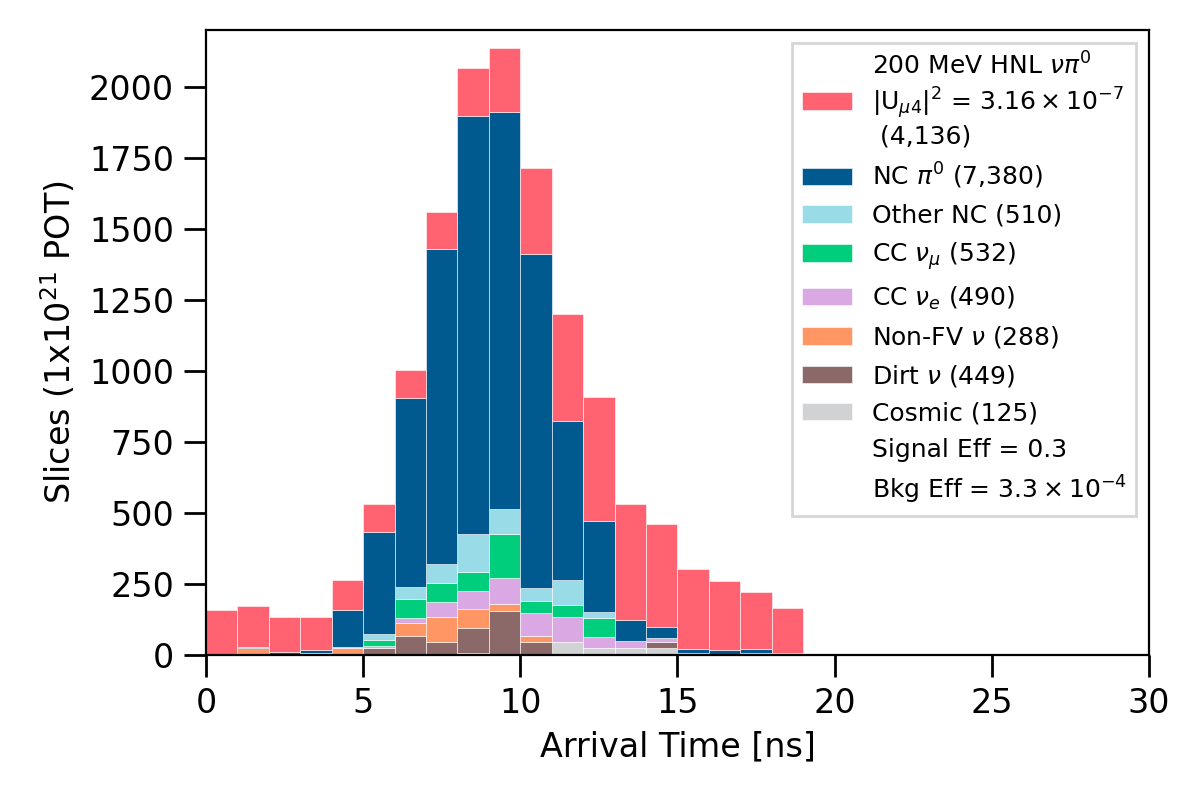
\includegraphics[width=\textwidth]{bb_lenient_full}
            \caption{Lenient cut: Full distribution}%
	    \label{fig:bb_full_loose}
        \end{subfigure}
        \hfill
	\begin{subfigure}[b]{0.495\textwidth}   
            \centering 
            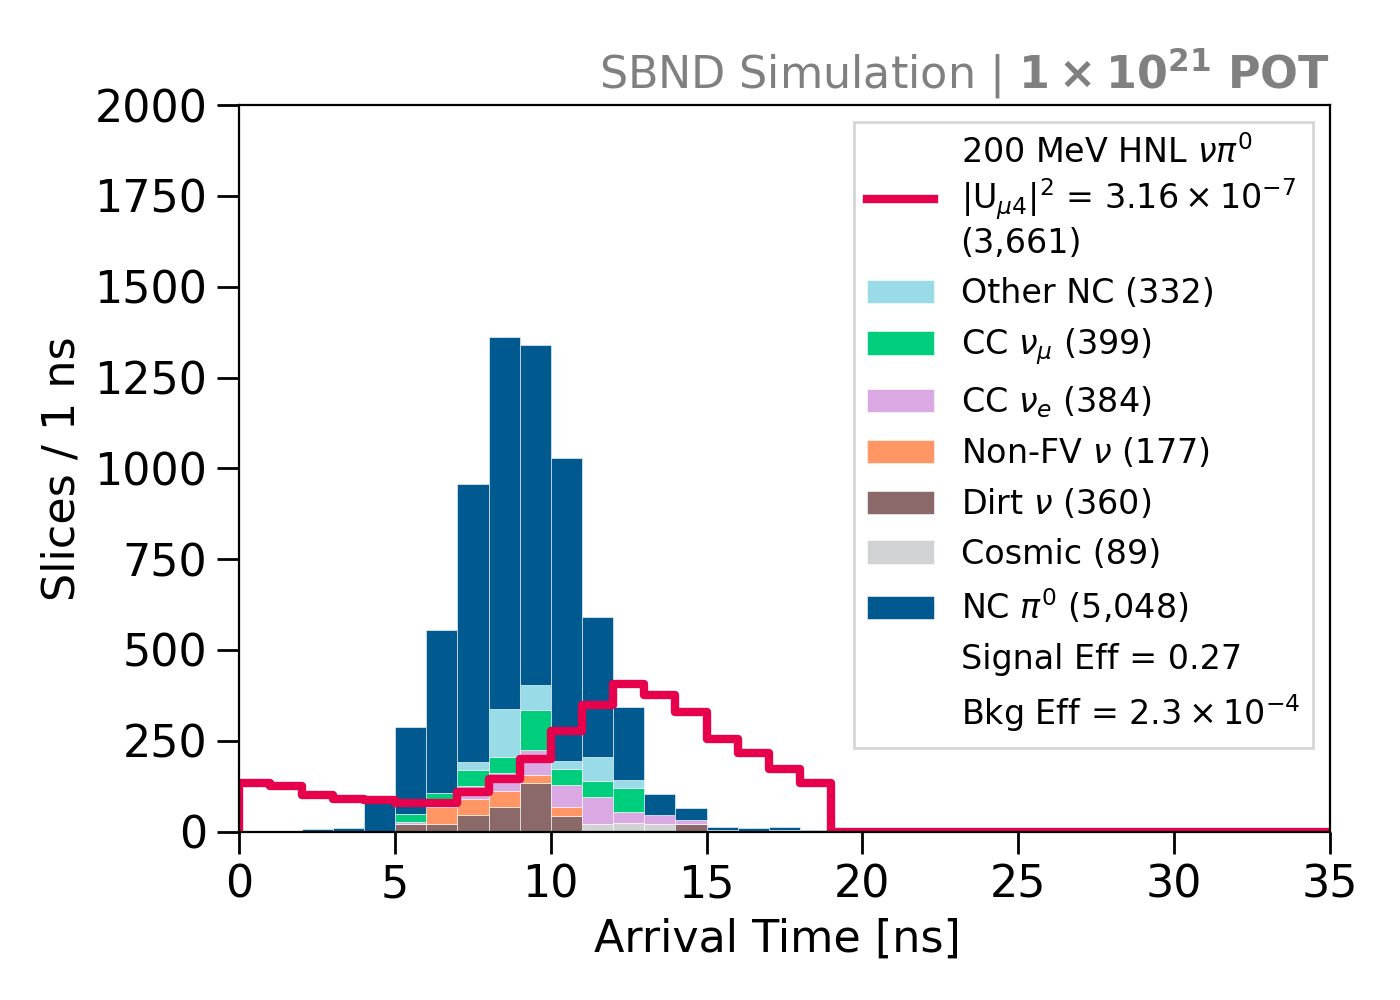
\includegraphics[width=\textwidth]{bb_stringent_full}
            \caption{Stringent cut: Full distribution}%
	    \label{fig:bb_full_strict}
        \end{subfigure}
	\hfill
        \begin{subfigure}[b]{0.495\textwidth}   
            \centering 
	    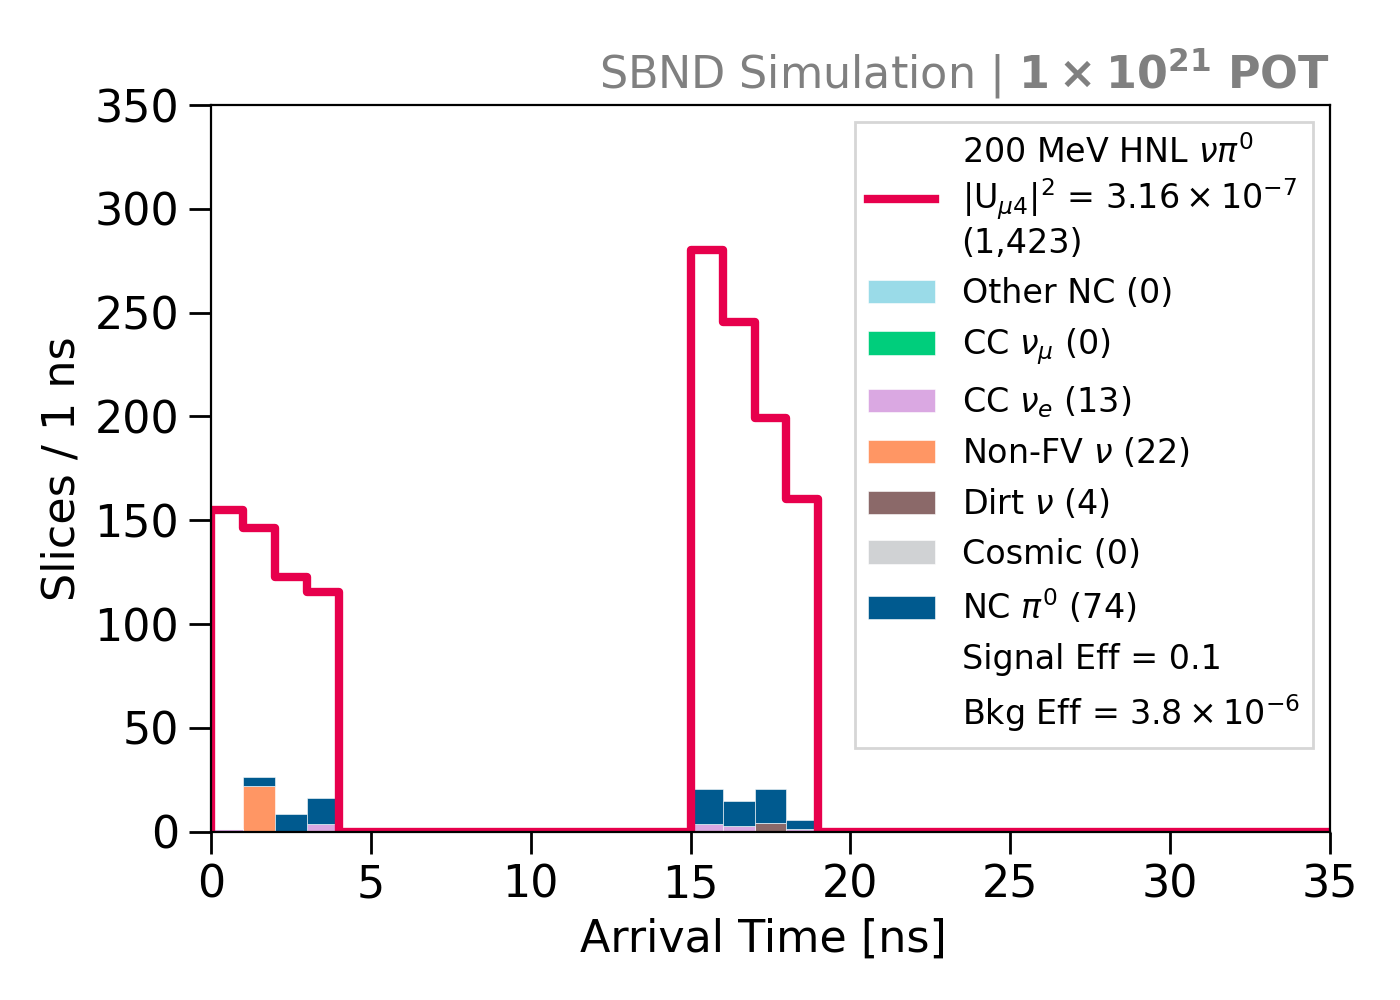
\includegraphics[width=\textwidth]{bb_lenient_edge}
            \caption{Lenient cut: Edge bins}%
	    \label{fig:bb_edge_loose}
        \end{subfigure}
        \hfill
        \begin{subfigure}[b]{0.495\textwidth}   
            \centering 
	    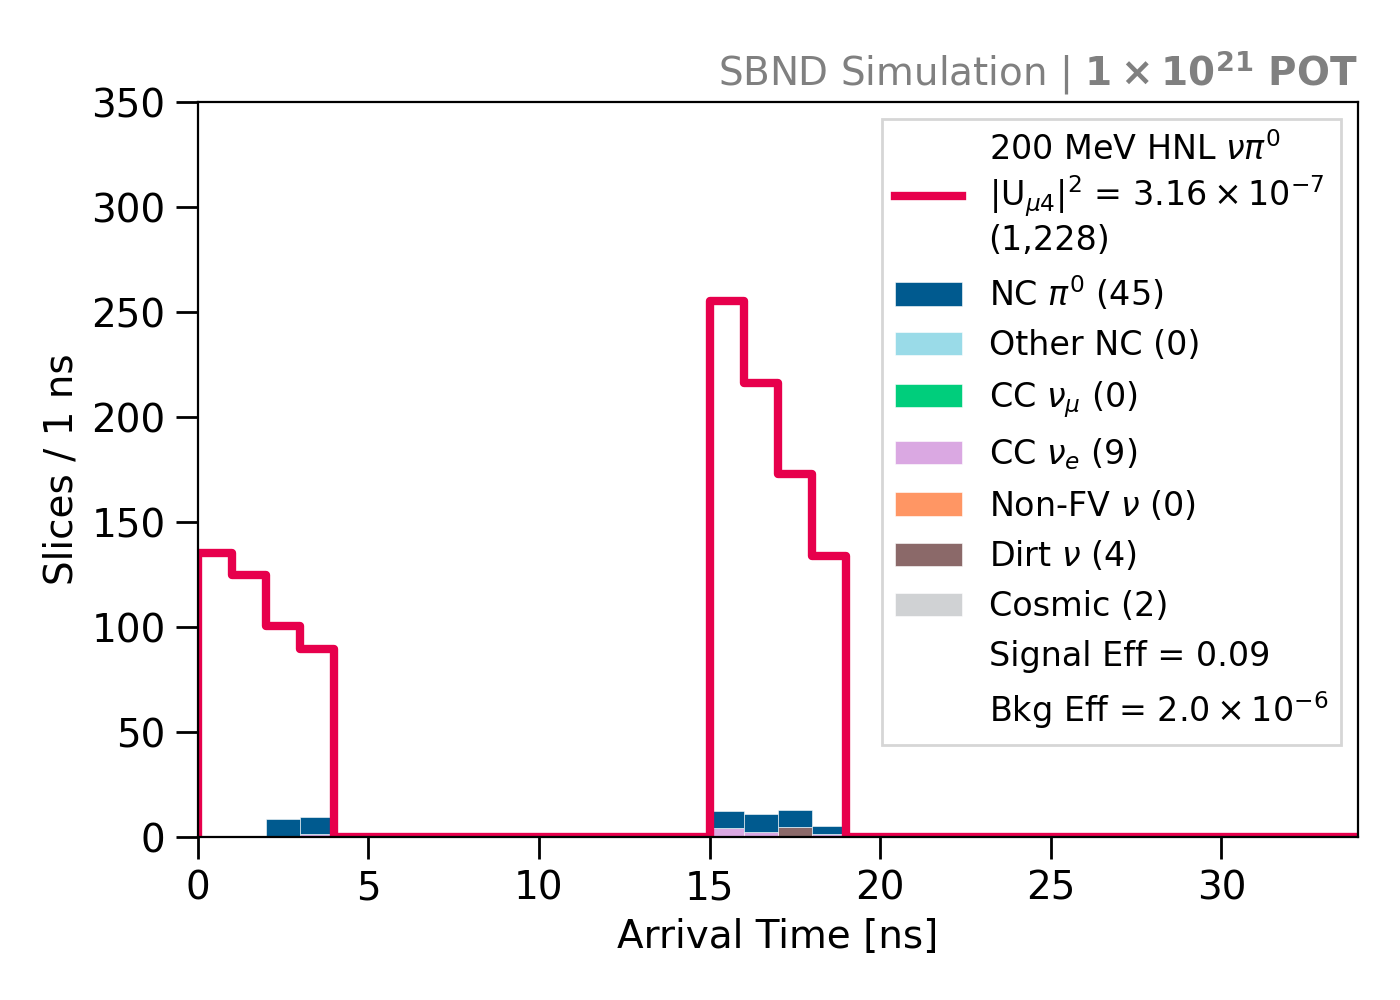
\includegraphics[width=\textwidth]{bb_stringent_edge}
            \caption{Stringent cut: Edge bins}%
	    \label{fig:bb_edge_strict}
        \end{subfigure}
	\caption[Arrival Time Distributions After Selection]{
	Arrival time distributions after the lenient (left) and stringent cut (right).
	}
        \label{fig:timing_cut}
\end{figure}

Fig. \ref{fig:eff} shows the signal and background rejection efficiency cut by cut.
The signal efficiency, Eq. \ref{eq:sig_eff}, is plotted using the left axis in pink and the background efficiency, Eq. \ref{eq:bkg_eff}, is plotted using the right axis in blue.
It is important to note that the right axis is in the logarithm scale as the background rejection is very aggressive.
The band of signal efficiency corresponds to the efficiency across the entire mass range of HNLs from 140 to 260 MeV, with efficiency increasing with masses. 
The selection differs from the calorimetry cut onwards, where the lenient cut is shown in solid line and the stringent cut is shown in dotted line.
Overall, the most significant cuts are the muon/proton/pion cut for track removal, followed by the calorimetry and theta angle cut by exploiting the boosted topology of HNLs that significantly reject backgrounds without compromising signal efficiency.

\begin{figure}[ht!]
    \centering 
    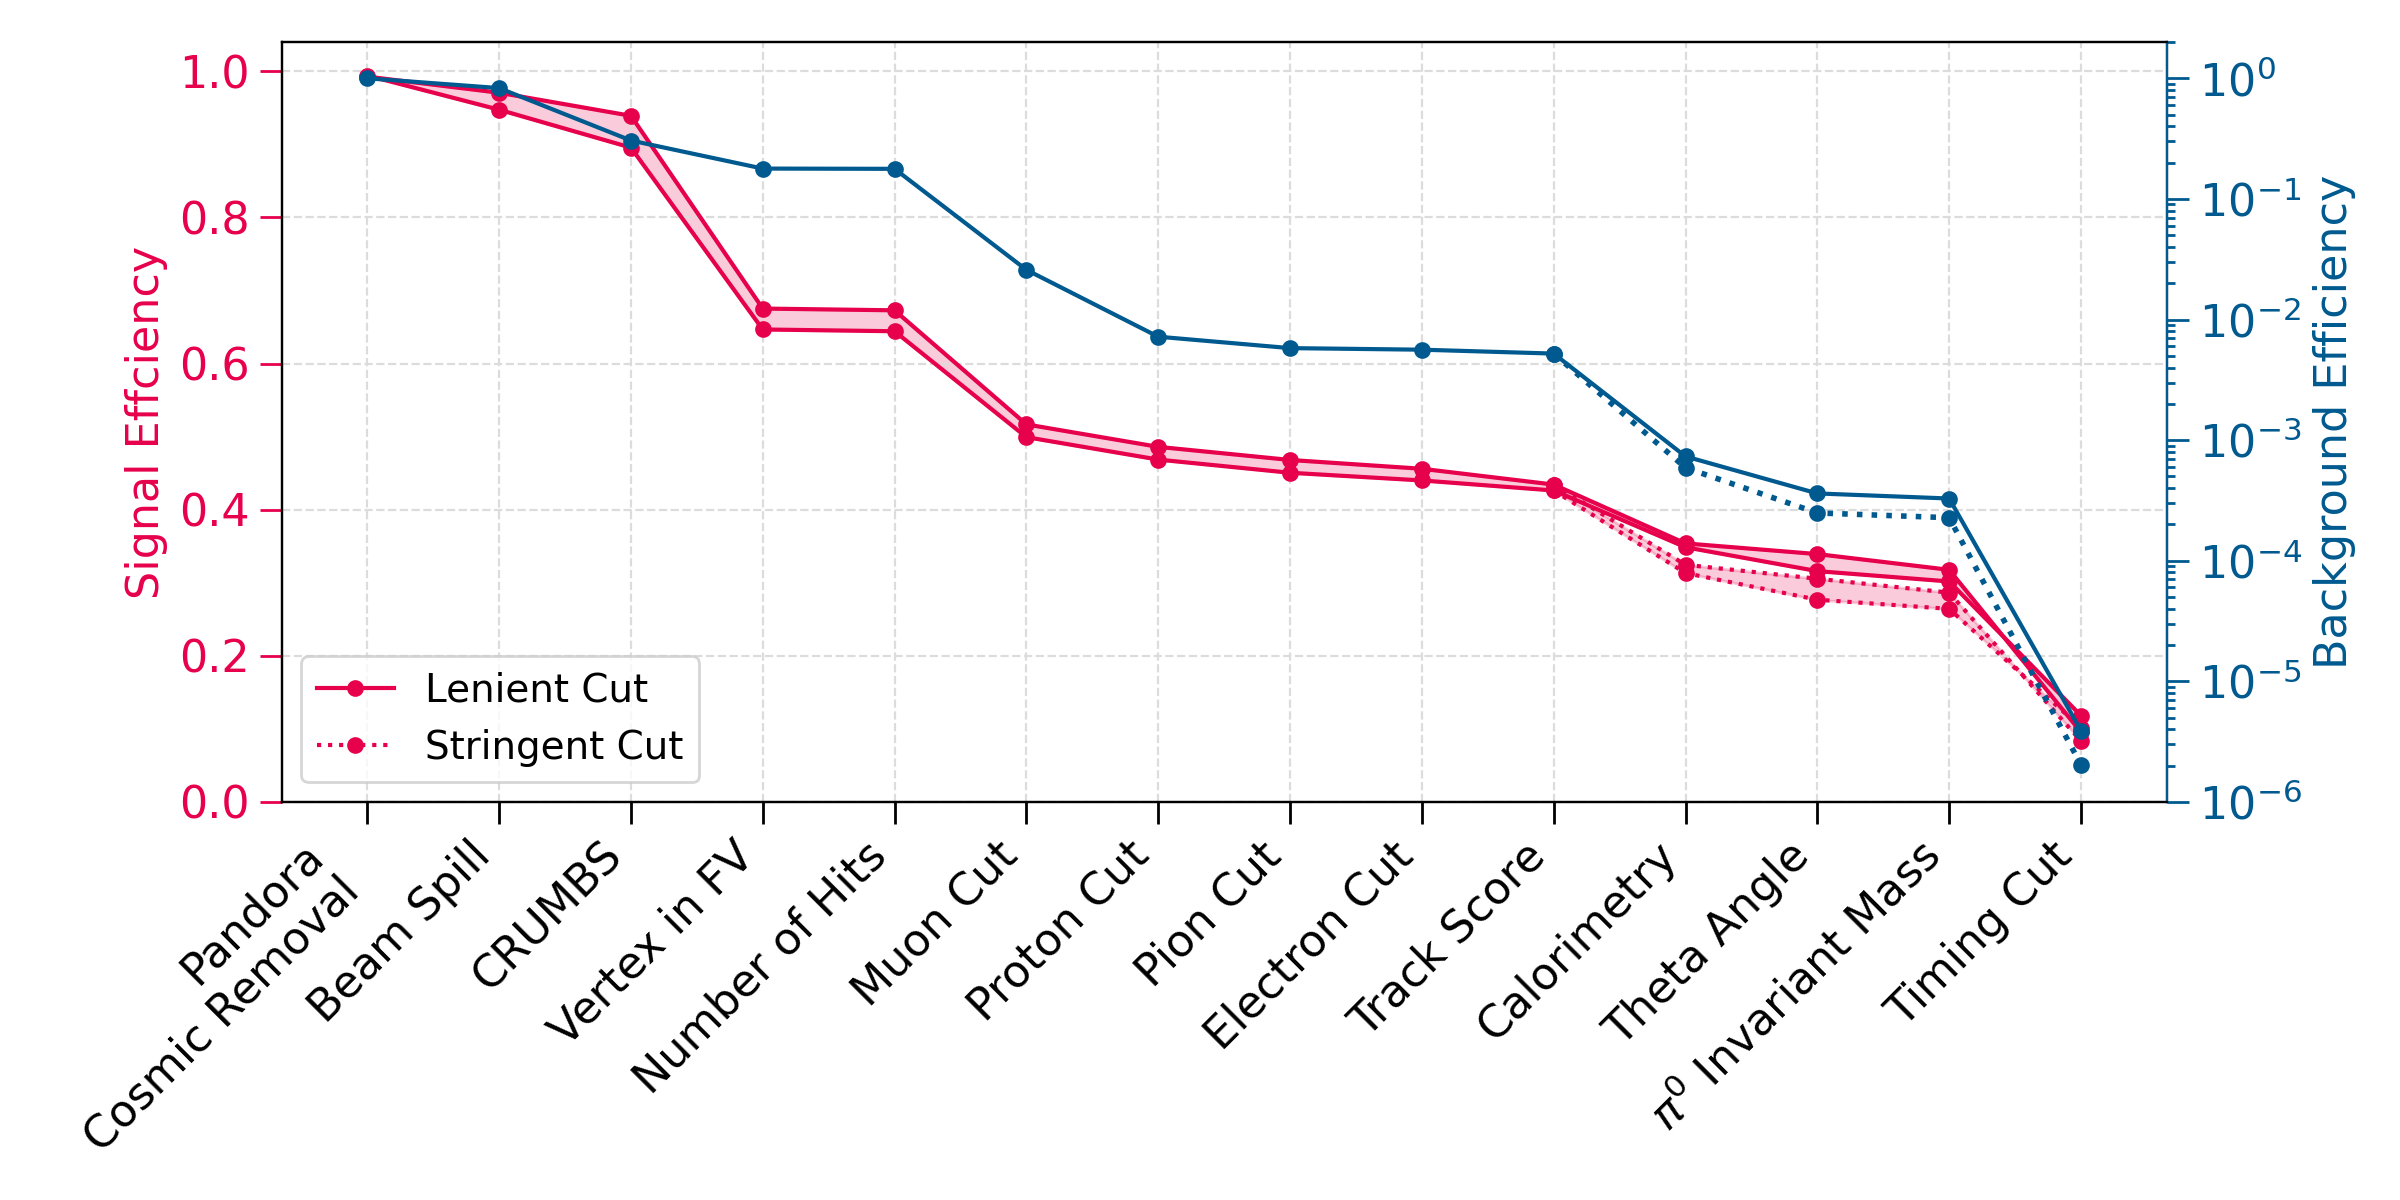
\includegraphics[width=1.0\textwidth]{peff_band}
    \caption[Summary of Selection Efficiency.]{
		Summary of signal (left axis) and background efficiencies (right axis).
	}
        \label{fig:eff}
\end{figure}


%********************************** %First Section  **************************************
\section{Study of Timing Resolution Improvement}
\label{sec:truth_bucket}

The timing cut described above demonstrates the importance of a high precision timing reconstruction in this analysis and thus, a study was carried out to understand the smearing contributors to the arrival time distribution. 
Fig. \ref{fig:smearing_factors} illustrates several factors that can smear the arrival time of a SM neutrino at SBND, and consequently smearing the Gaussian shape of the bucket.
The intrinsic Gaussian width of the proton bucket from the Booster synchrotron is 1.308 ns, as shown by the brown arrow (See Section \ref{sec4BNB}).
This structure is then smeared out due to the time of secondary mesons $t_{\mathrm{meson}}$, accounting for their interaction time and time of flight, as shown by the blue arrow.
The time of flight of the tertiary SM neutrinos from the production location to the detector $t_{\nu\ \mathrm{to\ detector}}$ further smears the Gaussian, as shown by the pink arrow.

Once the neutrino arrives at the detector, two additional smearing factors need to be considered.
The first one is its time of flight inside the detector until the interaction vertex $t_{\nu\ \mathrm{inside\ detector}}$, as shown by the purple arrow.
The second one is the time of flight of the photon from the production to the detection location $t_{\gamma}$, assuming the photon production location is close to the interaction vertex, as shown by the green arrow.

\begin{figure}[h!]
    \centering
    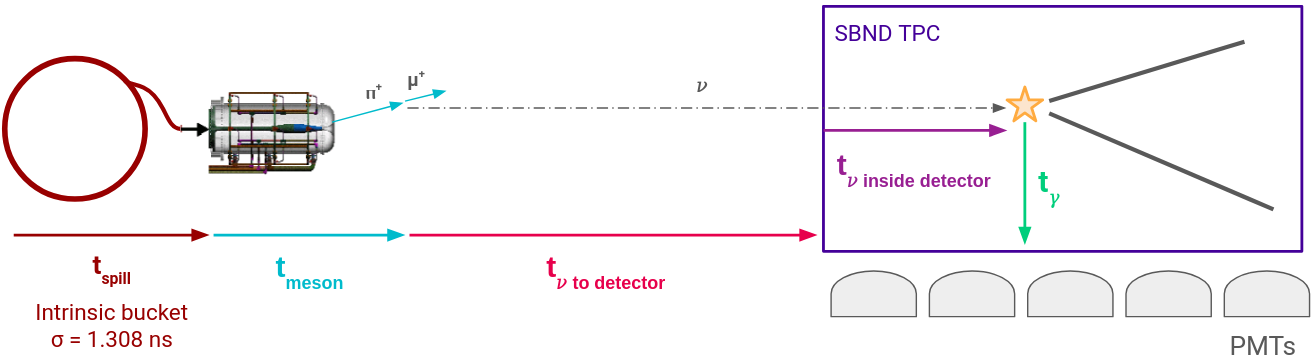
\includegraphics[width=1.0\textwidth]{smearing_factors.png}
    \caption[Smearing Contributors to the Arrival Time]{Diagram showing smearing contributors to the arrival time.}
    \label{fig:smearing_factors}
\end{figure}

\begin{figure}[b!]
    \centering
    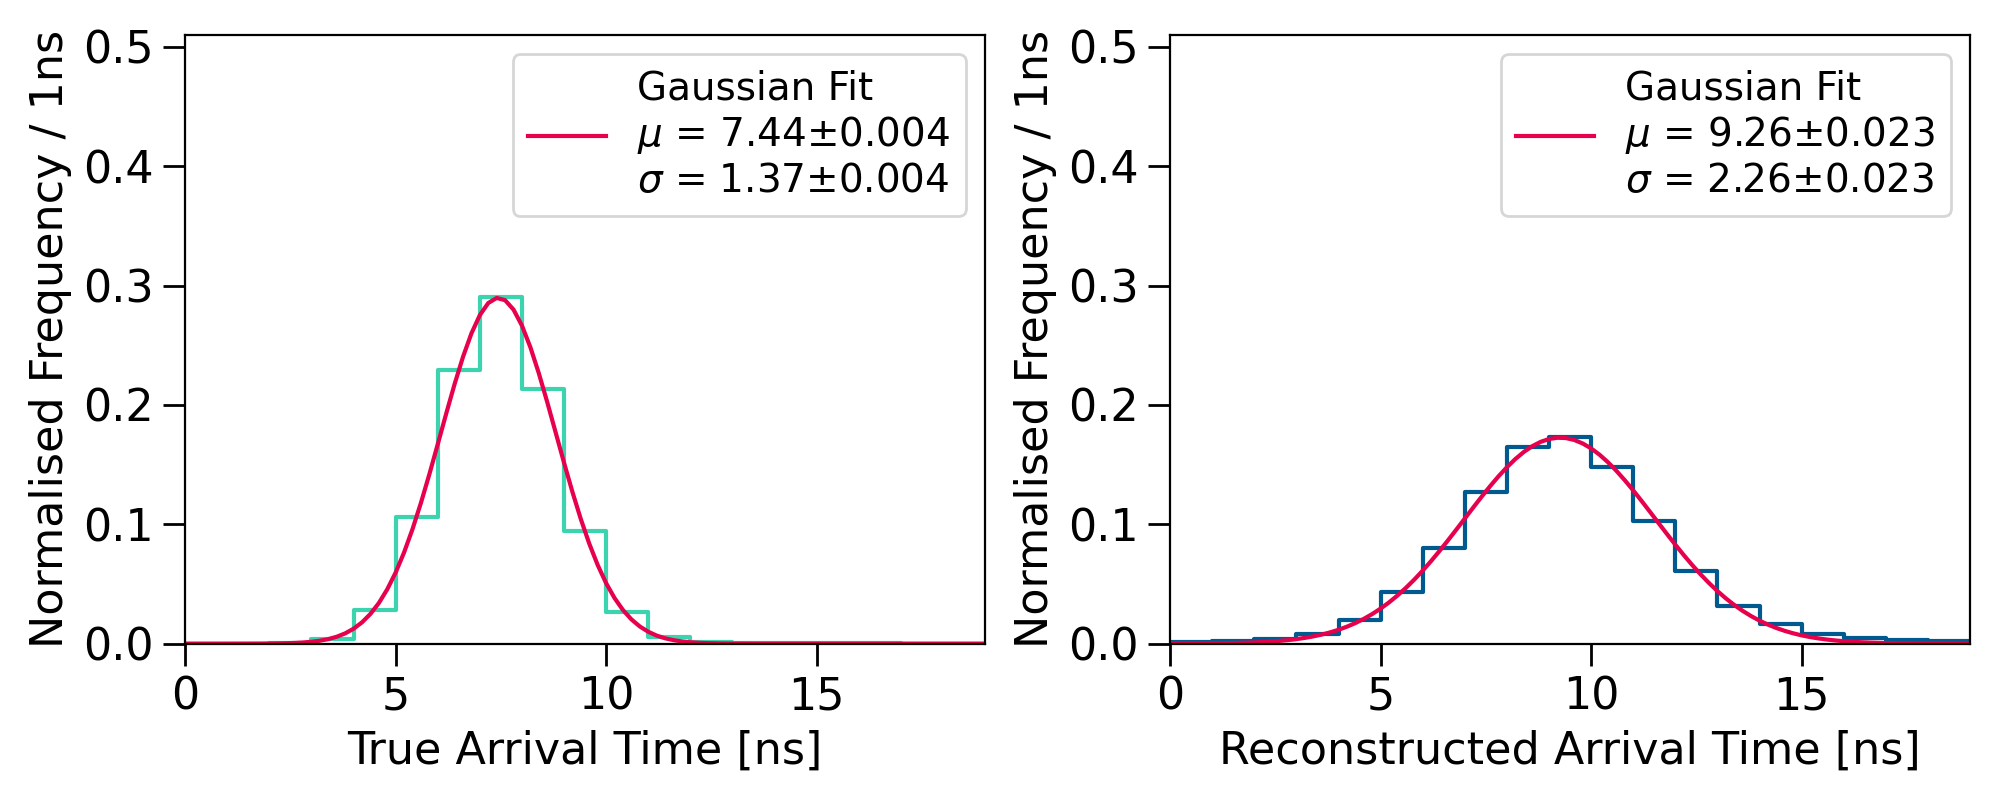
\includegraphics[width=0.75\textwidth]{truth_reco_gaus.png}
    \caption[Arrival Time of SM Neutrinos from True and Reconstructed Variables]{
    Arrival time distributions of SM neutrinos from true (left) and reconstructed variables (right).
    }
    \label{fig:gaus_truth_reco}
\end{figure}

The true arrival time distribution of SM neutrinos is shown in the left of Fig. \ref{fig:gaus_truth_reco}, where true indicates that no detector simulation and reconstruction are applied.
This distribution was computed using the true interaction time at the vertex, marked by the yellow star in Fig. \ref{fig:smearing_factors}, and corrected for $t_{\nu\ \mathrm{inside\ detector}}$.
It is can be seen that the combination of $t_{\mathrm{meson}}$ and $t_{\nu\ \mathrm{to\ detector}}$ smears the Gaussian width by a negligible amount from 1.308 ns to 1.37 ns.

The reconstructed arrival time distribution of SM neutrinos is depicted in the right of Fig. \ref{fig:gaus_truth_reco}.
The arrival time was computed from the flash time matched to a slice (See Sections \ref{sec:reco_pds} and \ref{sec:subsystem_match}).
The flash time was reconstructed using the prompt light in the first 30 ns window so that the scintillation location is close to the interaction vertex, and was also corrected for $t_{\gamma}$. 
The correction for $t_{\nu\ \mathrm{inside\ detector}}$ was applied by a shift from the reconstructed vertex $z$-position to $z = 0$ at the detector's front face.
As a result, the reconstruction depends on three variables: (1) the matching of slice-to-flash, (2) the flash time and (3) the slice vertex.
Each of these variables has its own reconstruction uncertainty, adding more smearing to the reconstructed arrival time.
%smearing the Gaussian shape of SM neutrinos arriving at the detector.
%The resulting arrival time corresponds to a Gaussian with a width smeared from 1.308 ns to 2.26 ns.

%The right figure was made using the Rockbox sample, selecting only slices that match a true neutrino. 
%No cosmic slices are considered for simplification, however, having cosmics background can additionally smear the structure.
%Both truth and reco plots are normalised for direct comparison.

Comparing the two distributions in Fig. \ref{fig:gaus_truth_reco}, the Gaussian mean is shifted by 1.82 ns from 7.44 to 9.26 ns.
This includes a shift of 1.45 ns introduced by the light reconstruction \cite{sbnd_pds_paper}.
The rest might be due to the slice vertex reconstruction and/or the slice-to-flash matching.      
Additionally, the Gaussian width is smeared from 1.37 ns to 2.26 ns. 
The width smearing is detrimental to the HNL search since it results in more SM neutrinos in the edge bins of the distribution, reducing the signal-to-background ratio in this region.  

This motivates the assessment of sensitivity assuming a better timing reconstruction.
The two assumptions of the arrival time distribution reconstructed with an improved timing resolution are as follows:
\begin{enumerate}
    \item A shifted Gaussian mean of 1.45 ns,
    \item A smeared Gaussian width of 1.73 ns.
\end{enumerate}
The first assumption is motivated by the impact of the light reconstruction in SBND reported in Ref. \cite{sbnd_pds_paper}.
The second assumption is motivated by the MicroBooNE experiment reporting on their intrinsic timing resolution in Ref. \cite{uboone_ns}.
Although ambitious, it is an achievable goal for SBND to have a reconstructed timing resolution $< 2$ ns, given that SBND employs a similar detector technology to MircoBooNE.
Moreover, Chapter \ref{ChapterDAQ} details the excellent timing performance of the SBND data acquisition and the preparation that already took place to achieve a better timing resolution.
Particularly, the SPEC-TDC device, as discussed in Section \ref{subsec42TimeRef}, records important timing information of triggers and beam arrivals that can only improve downstream reconstruction once incorporated. 

%To compare the smeared true to the reconstructed distribution \textit{after selection}, both distributions were normalised to same area.
%For example, the lenient selection leaves 9,761 background slices in the final distribution. 
%distributions normalised to the same area of the reconstructed distribution after selection. 
For modelling the background using true variables under these assumptions, only SM neutrinos are considered and not cosmics for simplicity. 
The true arrival time distribution of SM neutrinos was smeared with the two assumptions.
Fig. \ref{fig:gaus_truth_smear} shows the truth, smeared true and the reconstructed distribution after selection, normalised to the same area for direct comparison.
The left figure shows the true distribution without any smearing applied with a width of 1.37 ns.
The middle figure shows the smeared true distribution with the assumed width of 1.73 ns.
The right figure shows the reconstructed distribution after applying the lenient selection with a width of 1.99 ns.

\begin{figure}[ht!]
    \centering
    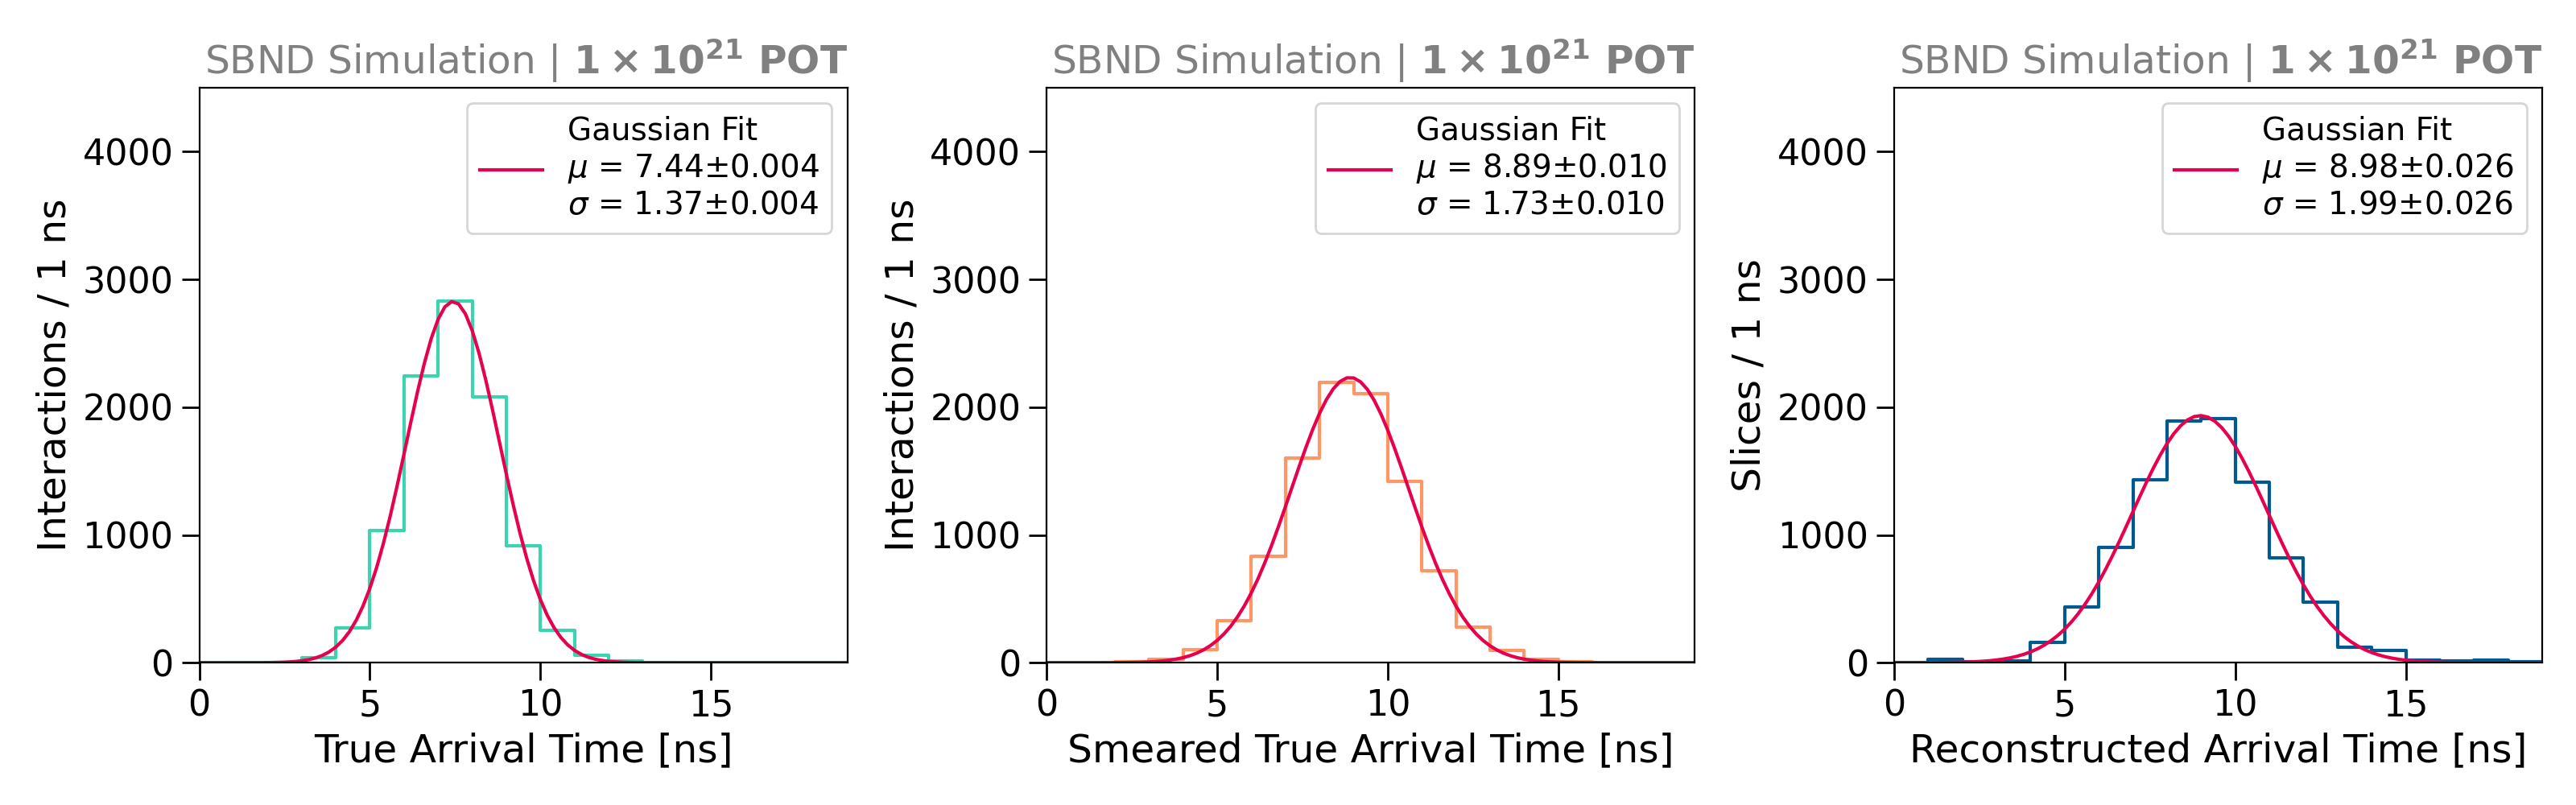
\includegraphics[width=\textwidth]{truth_smear_reco_gaus.png}
    \caption[Arrival Time of SM Neutrinos with an Improved Timing Resolution]{Arrival time distributions of SM neutrinos from true (left), smeared true (middle) and reconstructed variables after the lenient selection (right).}
    \label{fig:gaus_truth_smear}
\end{figure}


It is important to note the difference between the reconstructed arrival time before and after selection such that the distribution after selection has a less shifted Gaussian mean and a smaller Gaussian width.
It was observed in this work that different topologies have different timing reconstruction resolutions that result in slightly different Gaussian shapes. 
This might lead to cuts having non-uniform effects on the arrival time distribution.

For modelling the signal, the same smearing assumptions are applied to the true arrival time distribution of HNLs. 
%Unlike the background modelling approach of normalising the number of remaining background slices after selection, a flat efficiency of 30\% is applied to the HNL truth distribution to account for the effects of reconstruction and selection combined.
Unlike the background modelling approach of normalising the same area, an efficiency of 30\% was applied to the true distribution to account for the combined effects of reconstruction and selection.
Fig. \ref{fig:hnl_sm_smear} shows the arrival time distribution of SM neutrinos and HNLs from true, smeared true and reconstructed variables after selection for comparison. 
The smeared true distribution shows a higher signal-to-background ratio particularly for edge bins compared to the reconstructed distribution.
Thus, it is also used for determining the sensitivity alongside the reconstructed distributions in order to assess the impacts of timing resolution improvement.

\begin{figure}[ht!]
    \centering
    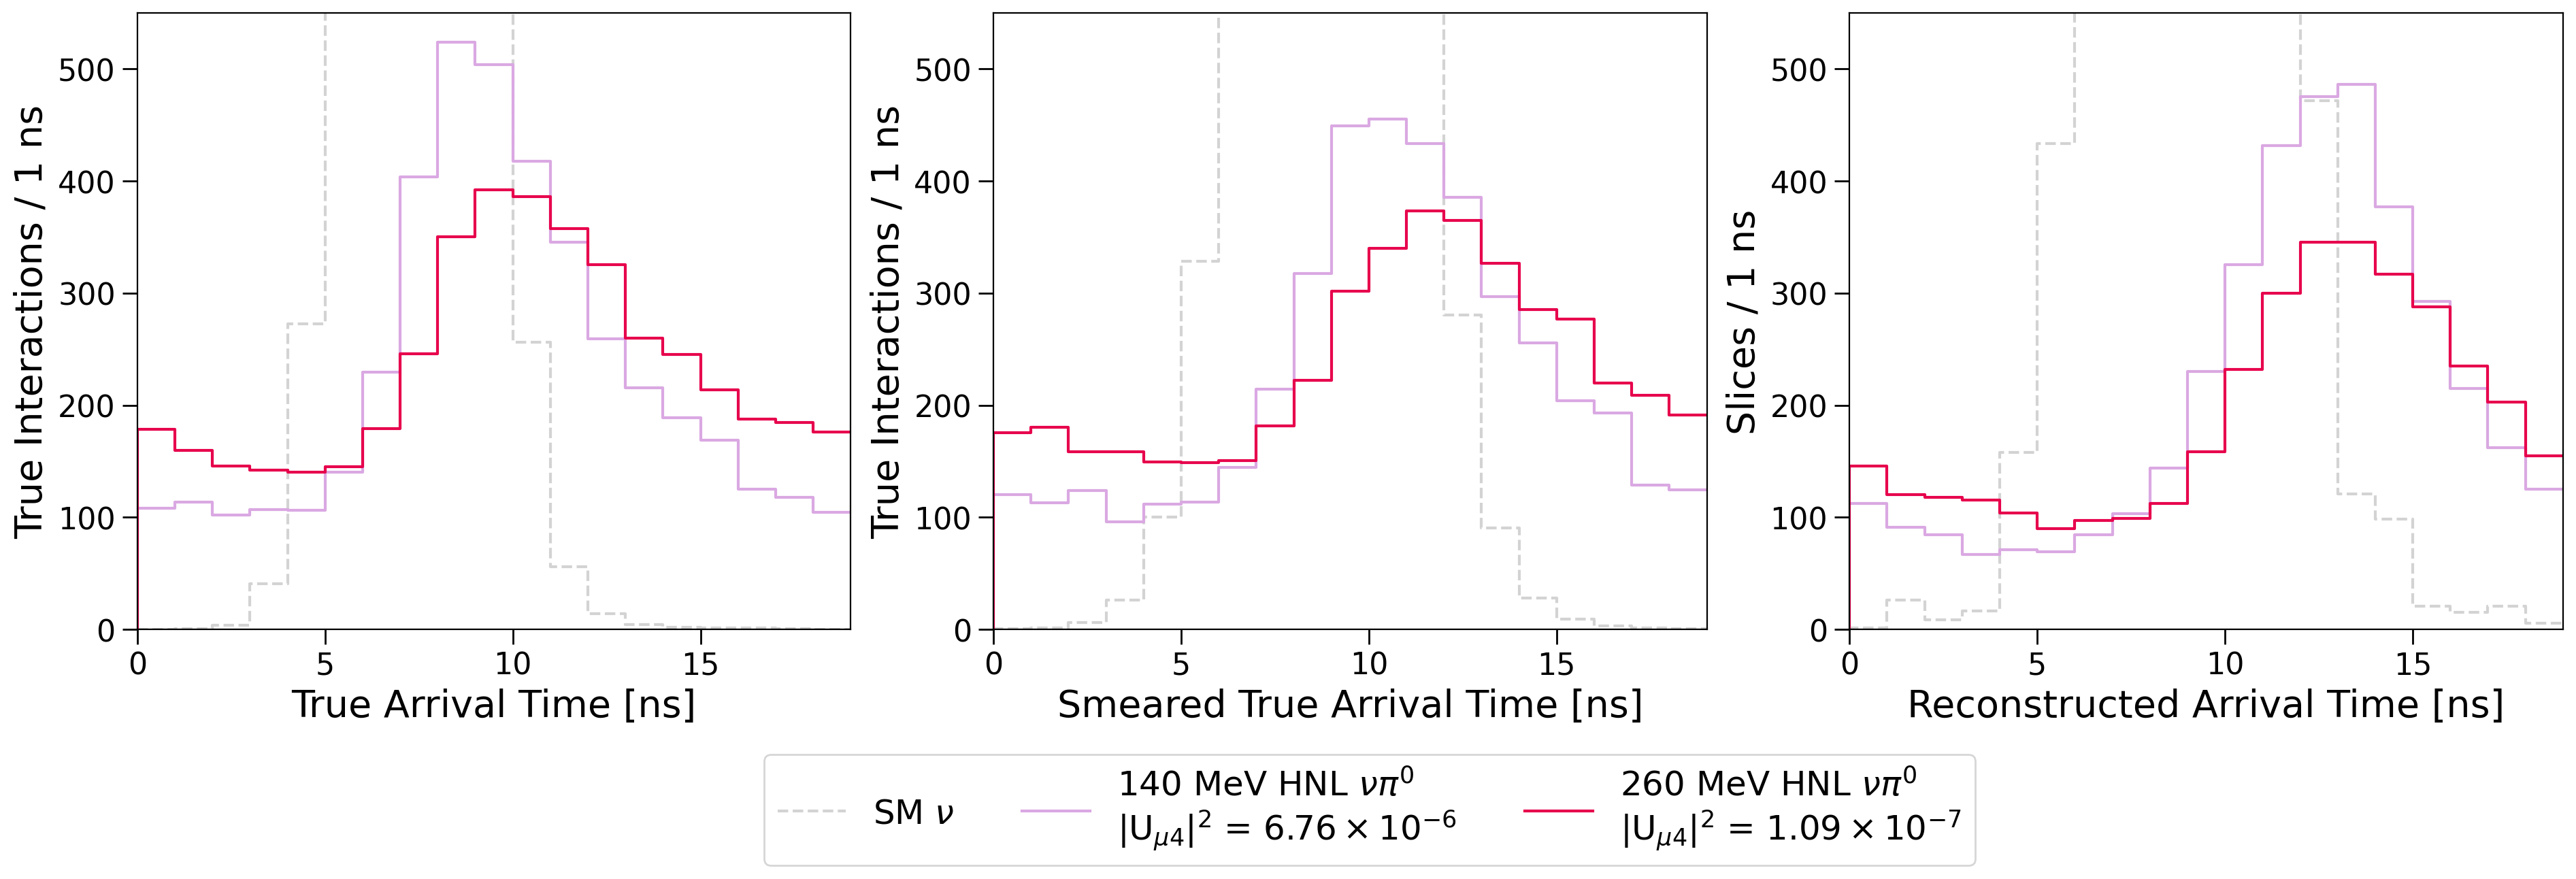
\includegraphics[width=\textwidth]{truth_smear_zoom.png}
    \caption[Arrival Time of SM Neutrinos and HNLs with an Improved Timing Resolution]{Arrival time distributions of SM neutrinos and HNLs from true (left), smeared true (middle) and reconstructed variables after the lenient selection (right).}
    \label{fig:hnl_sm_smear}
\end{figure}

%********************************** %First Section  **************************************

\section{Concluding Remarks}
\label{sec:select_conclude}

The selection of HNLs using MC samples is provided in this chapter, as a procedure to identify HNL signals from SM neutrino and cosmic backgrounds.
Two selection procedures on reconstructed variables are presented, the lenient and stringent cut, with the stringent rejecting backgrounds more aggressively than the lenient.
Both exploit the highly energetic and forward-going features of HNL showers to achieve an excellent background rejection without compromising signal efficiency.

The resulting background efficiency is in the order of $\mathcal{O}(10^{-4})$ while the signal selection efficiency still maintains at 30\%. 
When considering only bins at the edge of the arrival time distribution, or the so-called \textit{timing cut}, the background efficiency decreases significantly by two orders of magnitude to $\mathcal{O}(10^{-6})$.
Meanwhile, the signal efficiency only decreases from 30\% to 10\%. 
This demonstrates that these edge bins contain an exceptional signal-to-background ratio, which is the main factor driving the sensitivity.

Furthermore, a study was motivated to explore the impact on sensitivity if a better timing reconstruction is achieved.
The study resulted in a arrival time distribution acquired by smearing true variables, assuming it is reconstructed with an improved timing resolution of 1.73 ns compared to the current $\mathcal{O}$(2 ns).
All three arrival time distributions, from both the lenient and stringent cut on reconstructed variables and from the smeared true variables, are used for studying the sensitivity to HNLs in Chapter \ref{ChapterResult} next. 


%Thus, the signal-to-noise ratio varies bin-by-bin, where signal-rich bins locate at the edge of the arrival time (or the Gaussian tails) and background-rich bins locate at the centre of the arrival time (or the Gaussian peak).
%The setting limits procedure, to be detailed in upcoming Chapter \ref{ChapterResult}, employs a multi-binned analysis such that the resulting sensitivity limits depends on the signal-to-noise ratio per bin.
%This implies that signal-rich bins are the main factor driving the limits.
%With this in mind, the following selection procedure was optimised to achieve a high signal-to-noise ratio with bins located at the edge of the arrival time distribution.
